\documentclass[11pt,a4paper]{article}

% ── Packages ──────────────────────────────────────────────────────────
\usepackage[margin=2.4cm]{geometry}
\usepackage{amsmath}
\usepackage{amssymb}
\usepackage{graphicx}
\usepackage{booktabs}
\usepackage{longtable}
\usepackage{tabularx}
\usepackage{array}
\usepackage{hyperref}
\usepackage{xcolor}
\usepackage{tcolorbox}
\usepackage{titlesec}
\usepackage{enumitem}
\usepackage{microtype}
\usepackage{caption}
\usepackage{float}
\usepackage{parskip}
\captionsetup{font=small, labelfont=bf}

\hypersetup{
  colorlinks=true,
  linkcolor=blue!50!black,
  urlcolor=blue!50!black,
  citecolor=blue!50!black,
}

% Limitation box (red-tinted)
\newtcolorbox{limitbox}{
  colback=red!4, colframe=red!50!black, boxrule=0.5pt,
  arc=2pt, left=4pt, right=4pt, top=4pt, bottom=4pt,
  title=\textbf{Limitations}, fonttitle=\small\bfseries,
  coltitle=red!60!black, colbacktitle=red!10,
  before skip=8pt, after skip=8pt,
}

% Warning box (orange-tinted) for data flags
\newtcolorbox{warnbox}{
  colback=orange!5, colframe=orange!60!black, boxrule=0.5pt,
  arc=2pt, left=4pt, right=4pt, top=4pt, bottom=4pt,
  title=\textbf{Data warning}, fonttitle=\small\bfseries,
  coltitle=orange!60!black, colbacktitle=orange!15,
  before skip=8pt, after skip=8pt,
}

% Glossary box (blue-tinted)
\newtcolorbox{glossbox}[1]{
  colback=blue!4, colframe=blue!40!black, boxrule=0.5pt,
  arc=2pt, left=4pt, right=4pt, top=4pt, bottom=4pt,
  title=\textbf{#1}, fonttitle=\small\bfseries,
  coltitle=blue!60!black, colbacktitle=blue!10,
  before skip=8pt, after skip=8pt,
}

% Finding box (green-tinted)
\newtcolorbox{findbox}{
  colback=green!4, colframe=green!50!black, boxrule=0.5pt,
  arc=2pt, left=4pt, right=4pt, top=4pt, bottom=4pt,
  title=\textbf{Core finding}, fonttitle=\small\bfseries,
  coltitle=green!50!black, colbacktitle=green!10,
  before skip=8pt, after skip=8pt,
}

\titleformat{\section}{\Large\bfseries}{\thesection}{0.8em}{}
\titleformat{\subsection}{\large\bfseries}{\thesubsection}{0.7em}{}

% ── Title ─────────────────────────────────────────────────────────────
\title{\textbf{Trade-War Network Analysis:\\Preliminary Analysis Summary}}
\author{Olivia Peter \\ \small{Master Thesis, BSE}}
\date{May 2026}

\begin{document}

\maketitle
\tableofcontents
\vspace{1em}\hrule\vspace{1em}

% =====================================================================
\section{Overview}

This document summarises a preliminary exploratory analysis of how the global
trade network restructured around the US--China trade war (2018--2019) and
its aftermath. The work is organised in five phases:

\begin{itemize}[leftmargin=*]
  \item \textbf{Phase A} — Data foundation: harmonise the BACI bilateral trade
        panel with product-classification data (PLAID) and tariff data (FGKK).
  \item \textbf{Phase B} — Long-run network structure: compute year-by-year
        global network metrics on the aggregate trade network and on
        stage-stratified subnetworks (intermediate, capital, consumption,
        semiconductors).
  \item \textbf{Phase C} — Methodological honesty: visualise what the
        product-stage stratification adds over the aggregate-only view.
  \item \textbf{Phase D} — Tariff-stratified networks and friend-shoring
        analysis: trace the actual shift in US imports of tariffed products
        from China to other source countries, and inspect whether the
        connectors are doing genuine production or transshipping Chinese
        inputs.
  \item \textbf{Phase E} — Resilience analysis: apply four classical
        network-theoretic robustness measures to the aggregate network and
        each subnetwork, comparing the situation pre and post the trade war.
\end{itemize}

The remainder of this document explains each phase, the design decisions
that were taken, the core findings, and the limitations of what we can
defensibly conclude from the data.

% =====================================================================
\section{Research framing and a critical methodological note}

\subsection{Research questions}

Two related questions motivate the analysis:

\begin{enumerate}[label=(\arabic*),leftmargin=*]
  \item \textbf{Did US imports of tariffed products shift away from China toward
        connector countries (``friend-shoring'')?} And if so, are the
        connectors doing genuine production or simply re-routing Chinese
        intermediate inputs (``transshipment'')?
  \item \textbf{Did the global trade network become less resilient as a result
        of the trade war?} Specifically, did its topology become more fragile
        to hub failures, did the dense backbone shrink, or did the
        vulnerability profile change at the product-stage level?
\end{enumerate}

\subsection{What this analysis is — and is not}

A central methodological caveat applies throughout the document.

\begin{glossbox}{What we mean by ``GVC analysis from BACI''}
The CEPII BACI dataset records \textbf{gross} bilateral trade at HS6 product
level. A finished Vietnamese laptop shipped to the USA shows up as
\$200 of Vietnam$\to$USA trade. If half that laptop's value-added is in fact
a Korean chip embedded in it, BACI cannot tell us. The full GVC view
(``foreign value-added embedded in a flow'') requires \textbf{input-output tables}
(TiVA, OECD ICIO, EXIOBASE). We do not use those here.

What we do is partition gross-trade flows by product stage (intermediate /
capital / consumption, using PLAID's BEC classification). We then call the
intermediate-goods subnetwork our ``GVC-flavoured'' proxy. This is a defensible
shortcut, but it is a proxy, not a value-added decomposition.
\end{glossbox}

Throughout the document we are careful to phrase findings as
``what gross trade patterns reveal'' rather than ``what value-added flows reveal.''

% =====================================================================
\section{Phase A — Data foundation}

\subsection{Datasets}

\textbf{BACI HS92 V202601 (CEPII).} Bilateral trade flows in USD thousand,
disaggregated to the HS92 6-digit product code, covering 1995--2024 for
$\sim$230 countries. The HS92 vintage is used deliberately because CEPII
maintain consistency of the nomenclature for 30 years; newer products like
smartphones or lithium batteries are bundled into broader HS92 categories.

\textbf{PLAID v0.1 (Product-Level Attribute Indicator Database).} Five
HS6-level classifications of products:
\begin{itemize}[leftmargin=*]
  \item \texttt{bec}: UN Broad Economic Category — \emph{capital},
        \emph{intermediate}, \emph{consumption}, plus share columns.
  \item \texttt{rauch}: Rauch (1999) classification —
        \emph{differentiated} (branded, hard to substitute),
        \emph{reference-priced} (sold via reference prices),
        \emph{homogeneous} (commodity, sold on exchanges).
  \item \texttt{microchip\_content}: binary flag indicating whether the
        product contains electronics/microchips.
  \item \texttt{perishability}: shelf life and class.
  \item \texttt{hazmat}: hazardous-materials flag.
\end{itemize}
PLAID is built using the HS2022 revision (5{,}613 codes).

\textbf{FGKK 2023 tariff data.} From Fajgelbaum, Goldberg, Kennedy,
Khandelwal \& Taglioni's American Economic Review:~Insights paper, two
HS6-level tariff files:
\begin{itemize}[leftmargin=*]
  \item \texttt{z\_chus\_w}: Chinese retaliatory tariffs on US-origin
        imports, monthly 2018-04 to 2019-12 (8 event dates).
  \item \texttt{z\_usch\_w}: US Section 301 tariffs on Chinese imports,
        collapsed to three time periods $t \in \{-1, 0, 1\}$
        (pre / transition / post). 4{,}726 HS6 codes; max tariff +31\%
        weighted, +79\% stacked.
\end{itemize}

\textbf{OECD TiVA Foreign Direct Value Added (FDVA).} Country~$\times$~sector
value-added flows for 2019--2022, cached locally as
\texttt{tiva\_fdva\_cache/}. Not used in headline analyses but available for
future cross-validation.

\subsection{Building the combined panel}

The 30 yearly BACI CSVs are converted to per-year Parquet files (\textasciitilde85--90~MB each).
A streaming pipeline (\texttt{build\_baci\_artifacts.py}) processes them
year-by-year on a 16~GB machine without ever loading the full 19.7~GB into
memory. It produces:
\begin{itemize}[leftmargin=*]
  \item \texttt{baci\_combined.parquet} — 269.9~M rows of HS6-level
        bilateral flows enriched with ISO3 codes and HS2 chapter.
  \item \texttt{baci\_edges\_country.parquet} — 870{,}755 rows
        (year $\times$ source $\times$ target, aggregated across products).
\end{itemize}

\subsection{The BACI~$\leftrightarrow$~PLAID classification mismatch}

PLAID is in HS2022; BACI is in HS92. Direct HS6 merging gives only
\textbf{75\% trade-value coverage}. The missing 25\% is concentrated in
modern products — exactly the trade-war-relevant categories. To bridge the
gap we aggregate both to the HS4 chapter level (which is much more stable
across HS revisions): \textbf{99.4\% trade-value coverage} in 2017 and
\textbf{99.5\% in 2023}. Within-HS4 homogeneity of PLAID's BEC classification
is high (1{,}097 of 1{,}229 chapters have $\geq$80\% modal-class dominance).
This is the trade-off we accept: full coverage at HS4 granularity, with
chapter-averaged PLAID classifications.

\subsection{PLAID-stratified edge lists}

A second streaming pipeline (\texttt{build\_plaid\_edges.py}) merges the HS4
PLAID master onto each BACI row and \textbf{fractionally allocates} each trade
flow across product stages. For example, a flow in an HS4 chapter that is
80\% intermediate and 20\% capital gets split 80/20 between the two stages.
This preserves trade-value totals (no arbitrary cut-offs). Outputs:
\begin{itemize}[leftmargin=*]
  \item \texttt{baci\_edges\_country\_by\_bec.parquet} (2.6~M rows: 3 BEC stages)
  \item \texttt{baci\_edges\_country\_by\_rauch.parquet} (2.6~M rows: 3 Rauch classes)
  \item \texttt{baci\_edges\_country\_microchip.parquet} (1.7~M rows: microchip vs not)
\end{itemize}

\subsection{Tariff master}

The FGKK tariff variables are pivoted to one row per HS6 with the
post-period (\texttt{t=1}) tariff level and the change from baseline. An
HS4 aggregation is produced for joint use with PLAID. The combined master
\texttt{hs4\_master.csv} provides one row per HS4 chapter with all PLAID
classifications and the tariff-exposure summary.

\begin{limitbox}
\textbf{PLAID is v0.1} and we have no formal methodology document for it. We
take its HS6-level classifications at face value. The HS4-level aggregation
introduces small composition distortions for chapters with mixed BEC mixes
($\sim$11\% of chapters). The FGKK tariff data is restricted to the products
the authors tracked (4{,}726 HS6 codes); for the remaining BACI codes we
default to ``untreated.''
\end{limitbox}

% =====================================================================
\section{Phase B.1 — Long-run network structure (aggregate)}

\subsection{Network glossary — terms used throughout this section}

\begin{glossbox}{Network terms}
\textbf{Density}: number of actual edges divided by the maximum possible
edges. Tells you how connected the network is overall.

\textbf{Degree / strength}: a country's number of trade partners (degree) or
the total weight of its trade ties (strength). Out-strength = sum of exports;
in-strength = sum of imports.

\textbf{PageRank}: a centrality measure that weights a country by the
importance of the partners it trades with. Originally developed for Google
web-ranking.

\textbf{Betweenness centrality}: counts how often a country sits on the
shortest trade-routing path between other countries. High betweenness =
intermediary / hub role.

\textbf{Modularity (Louvain)}: a number between 0 and 1 measuring how cleanly
the network divides into communities. Higher = clearer bloc structure.

\textbf{HHI (Herfindahl--Hirschman Index)}: a concentration measure. Sum of
squared shares. 0 = perfectly diversified, 1 = monopoly. Used here to
measure how concentrated global exports are in a few countries.

\textbf{Jaccard similarity}: of two edge sets, the size of their intersection
over the size of their union. Used here year-over-year to measure
``how much the network's link structure changed.''
\end{glossbox}

\subsection{What we computed}

Using \texttt{long\_run\_network\_metrics.py}, for each year 1995--2024 we
built a directed weighted graph (nodes = countries, edges = bilateral
trade) and computed: density, modularity, Louvain communities,
out-strength HHI, edge-set Jaccard versus the previous year, and centrality
measures (PageRank, eigenvector, betweenness) for a watchlist of major
players. The pipeline outputs three CSVs:
\texttt{long\_run\_global\_metrics.csv},
\texttt{long\_run\_country\_metrics.csv},
\texttt{long\_run\_community\_assignments.csv}.

\subsection{Findings — aggregate network}

\begin{findbox}
\textbf{1. Slowbalization plateau is visible.} Network density rose
steadily from 0.24 (1995) to 0.34 (2010), then stayed flat through 2024.
The aggregate trade network stopped densifying around the time of the
post-GFC recovery.

\textbf{2. China is now the dominant network hub.} China's
out-strength share of global trade rose 4.5\% (1995) $\to$ 15.7\% (2024).
Its weighted betweenness centrality rose from 0.03 (1995) to 0.75 (2024)
— from peripheral to the network's primary intermediary.

\textbf{3. USA lost intermediary role.} USA's betweenness fell from 0.66
(1995) to 0.42 (2024), while its export share fell from 12.3\% to 8.2\%.

\textbf{4. Three stable blocs.} Louvain community detection consistently
identifies three communities since $\sim$2008: an Americas bloc
(USA, CAN, MEX, BRA initially), an Europe bloc (DEU, FRA, GBR, NLD,
\ldots), and an Asia-Pacific bloc (CHN, JPN, KOR, S19, VNM, IND, AUS,
\ldots). Brazil defected from the Americas bloc to the Asia-Pacific bloc
between 2017 and 2019 — visual evidence of China's commodity pull.

\textbf{5. Modularity declined slightly post-2008}, contradicting the
``trade war fragmented the network'' hypothesis. Number of communities
stayed at 3--4.

\textbf{6. Connector watchlist rise.} Vietnam's PageRank grew +21\%,
Brazil's +20\%, between 2017 and 2024. Japan declined the most ($-18\%$).
\end{findbox}

\begin{figure}[H]
  \centering
  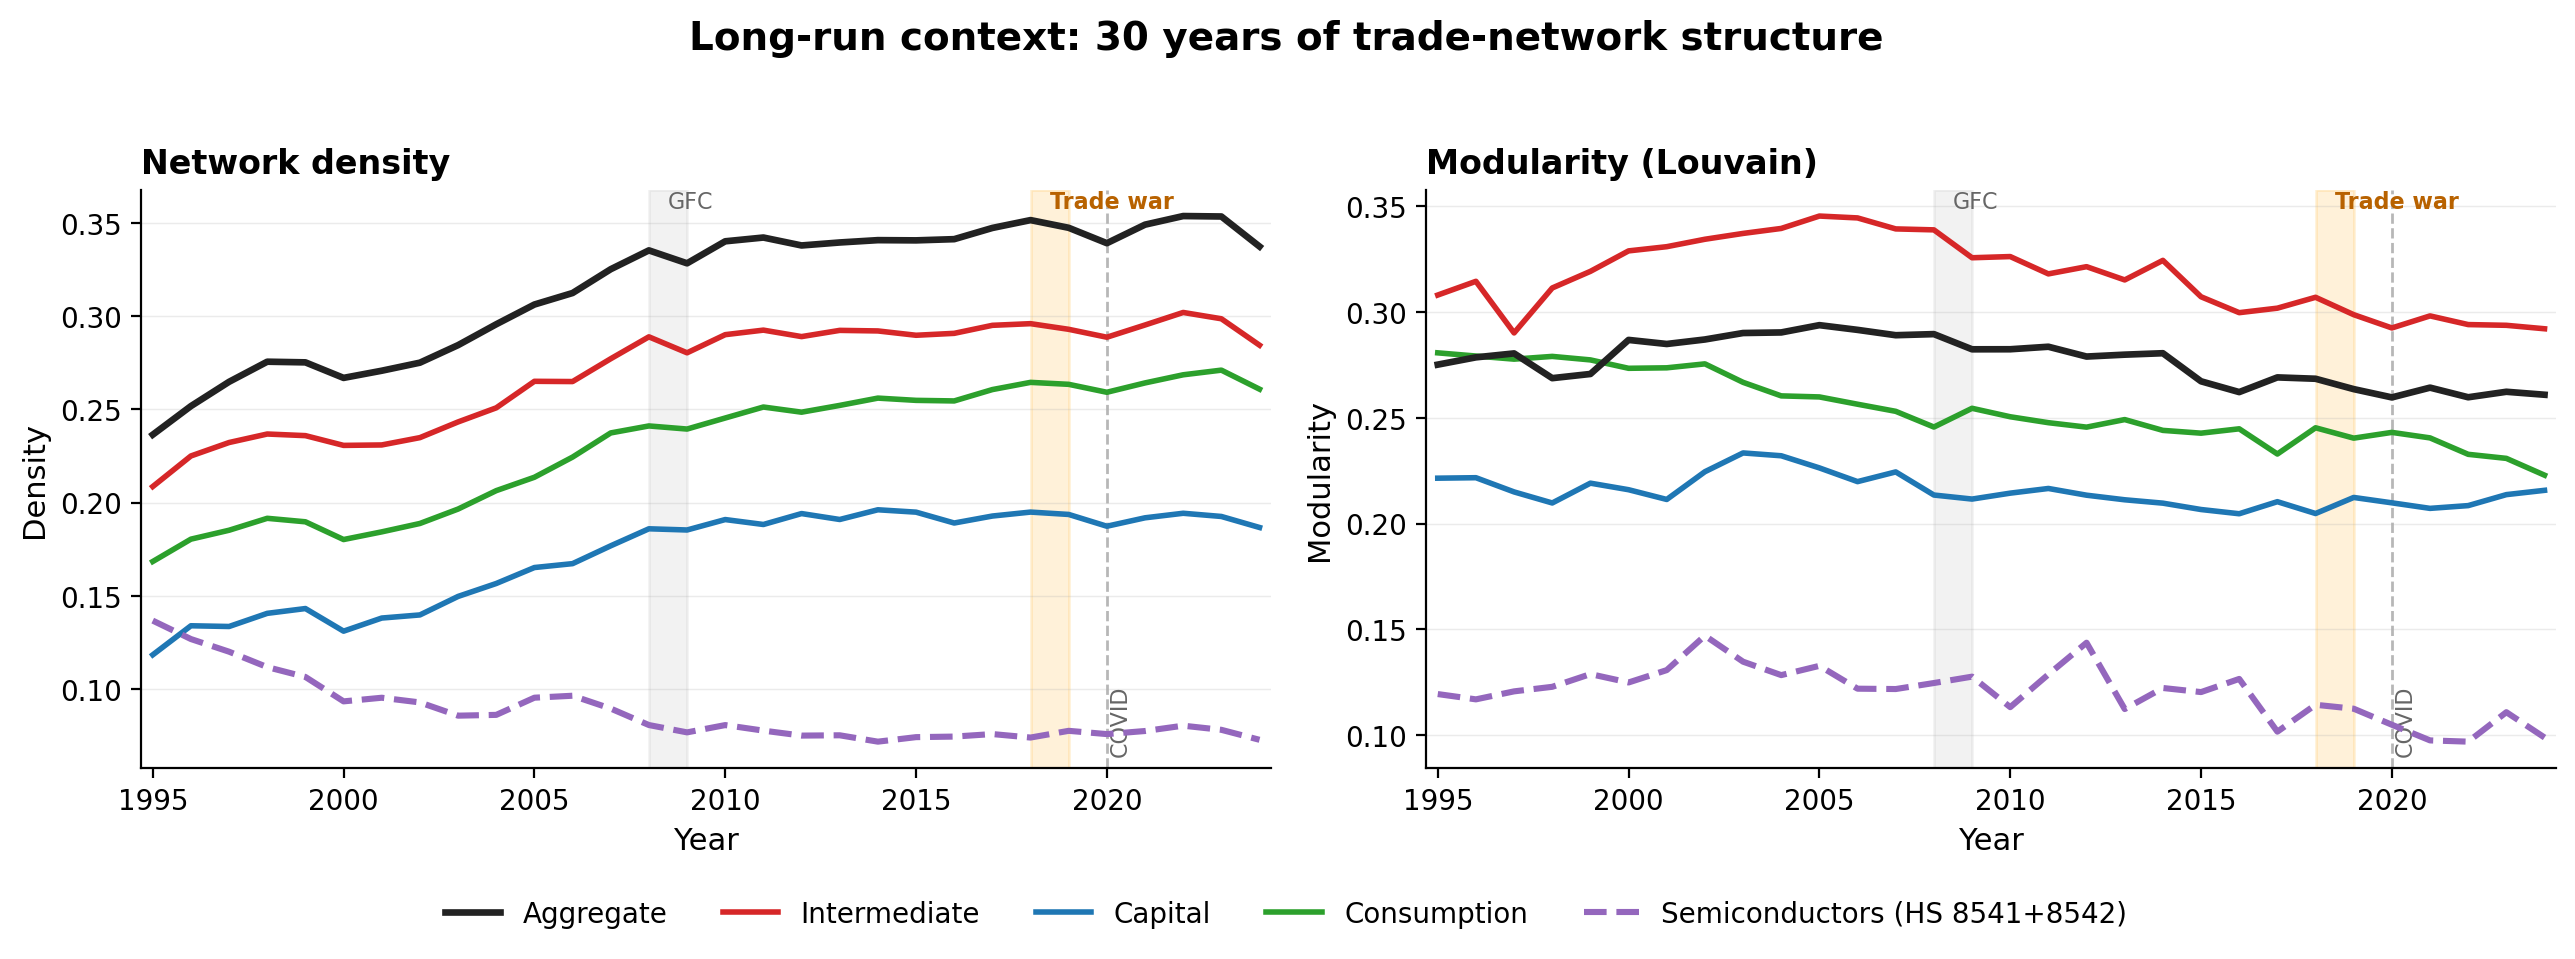
\includegraphics[width=\textwidth]{figures/fig4_long_run_context.png}
  \caption{Long-run context: density and modularity 1995--2024.
  Density plateaus after $\sim$2010; intermediate-goods modularity peaks
  around 2003--2007 and declines through the trade-war period.}
  \label{fig:longrun}
\end{figure}

\begin{limitbox}
The aggregate-network view captures \textit{compositional invariance}: total
trade can be flat while \textit{who exports what to whom} shifts dramatically.
The blocs are stable but countries reposition within them. Any conclusion
about ``the trade war did not fragment the network'' is correct at the
country-level country$\times$country aggregation but says nothing about
fragmentation \textit{within product stages}.
\end{limitbox}

% =====================================================================
\section{Phase B.2 — BEC-stratified networks}

The aggregate may hide patterns that show up at the product-stage level.
We re-ran the long-run pipeline on each BEC stage separately using
\texttt{long\_run\_metrics\_by\_bec.py}.

\subsection{Findings — BEC stages tell different stories}

\begin{figure}[H]
  \centering
  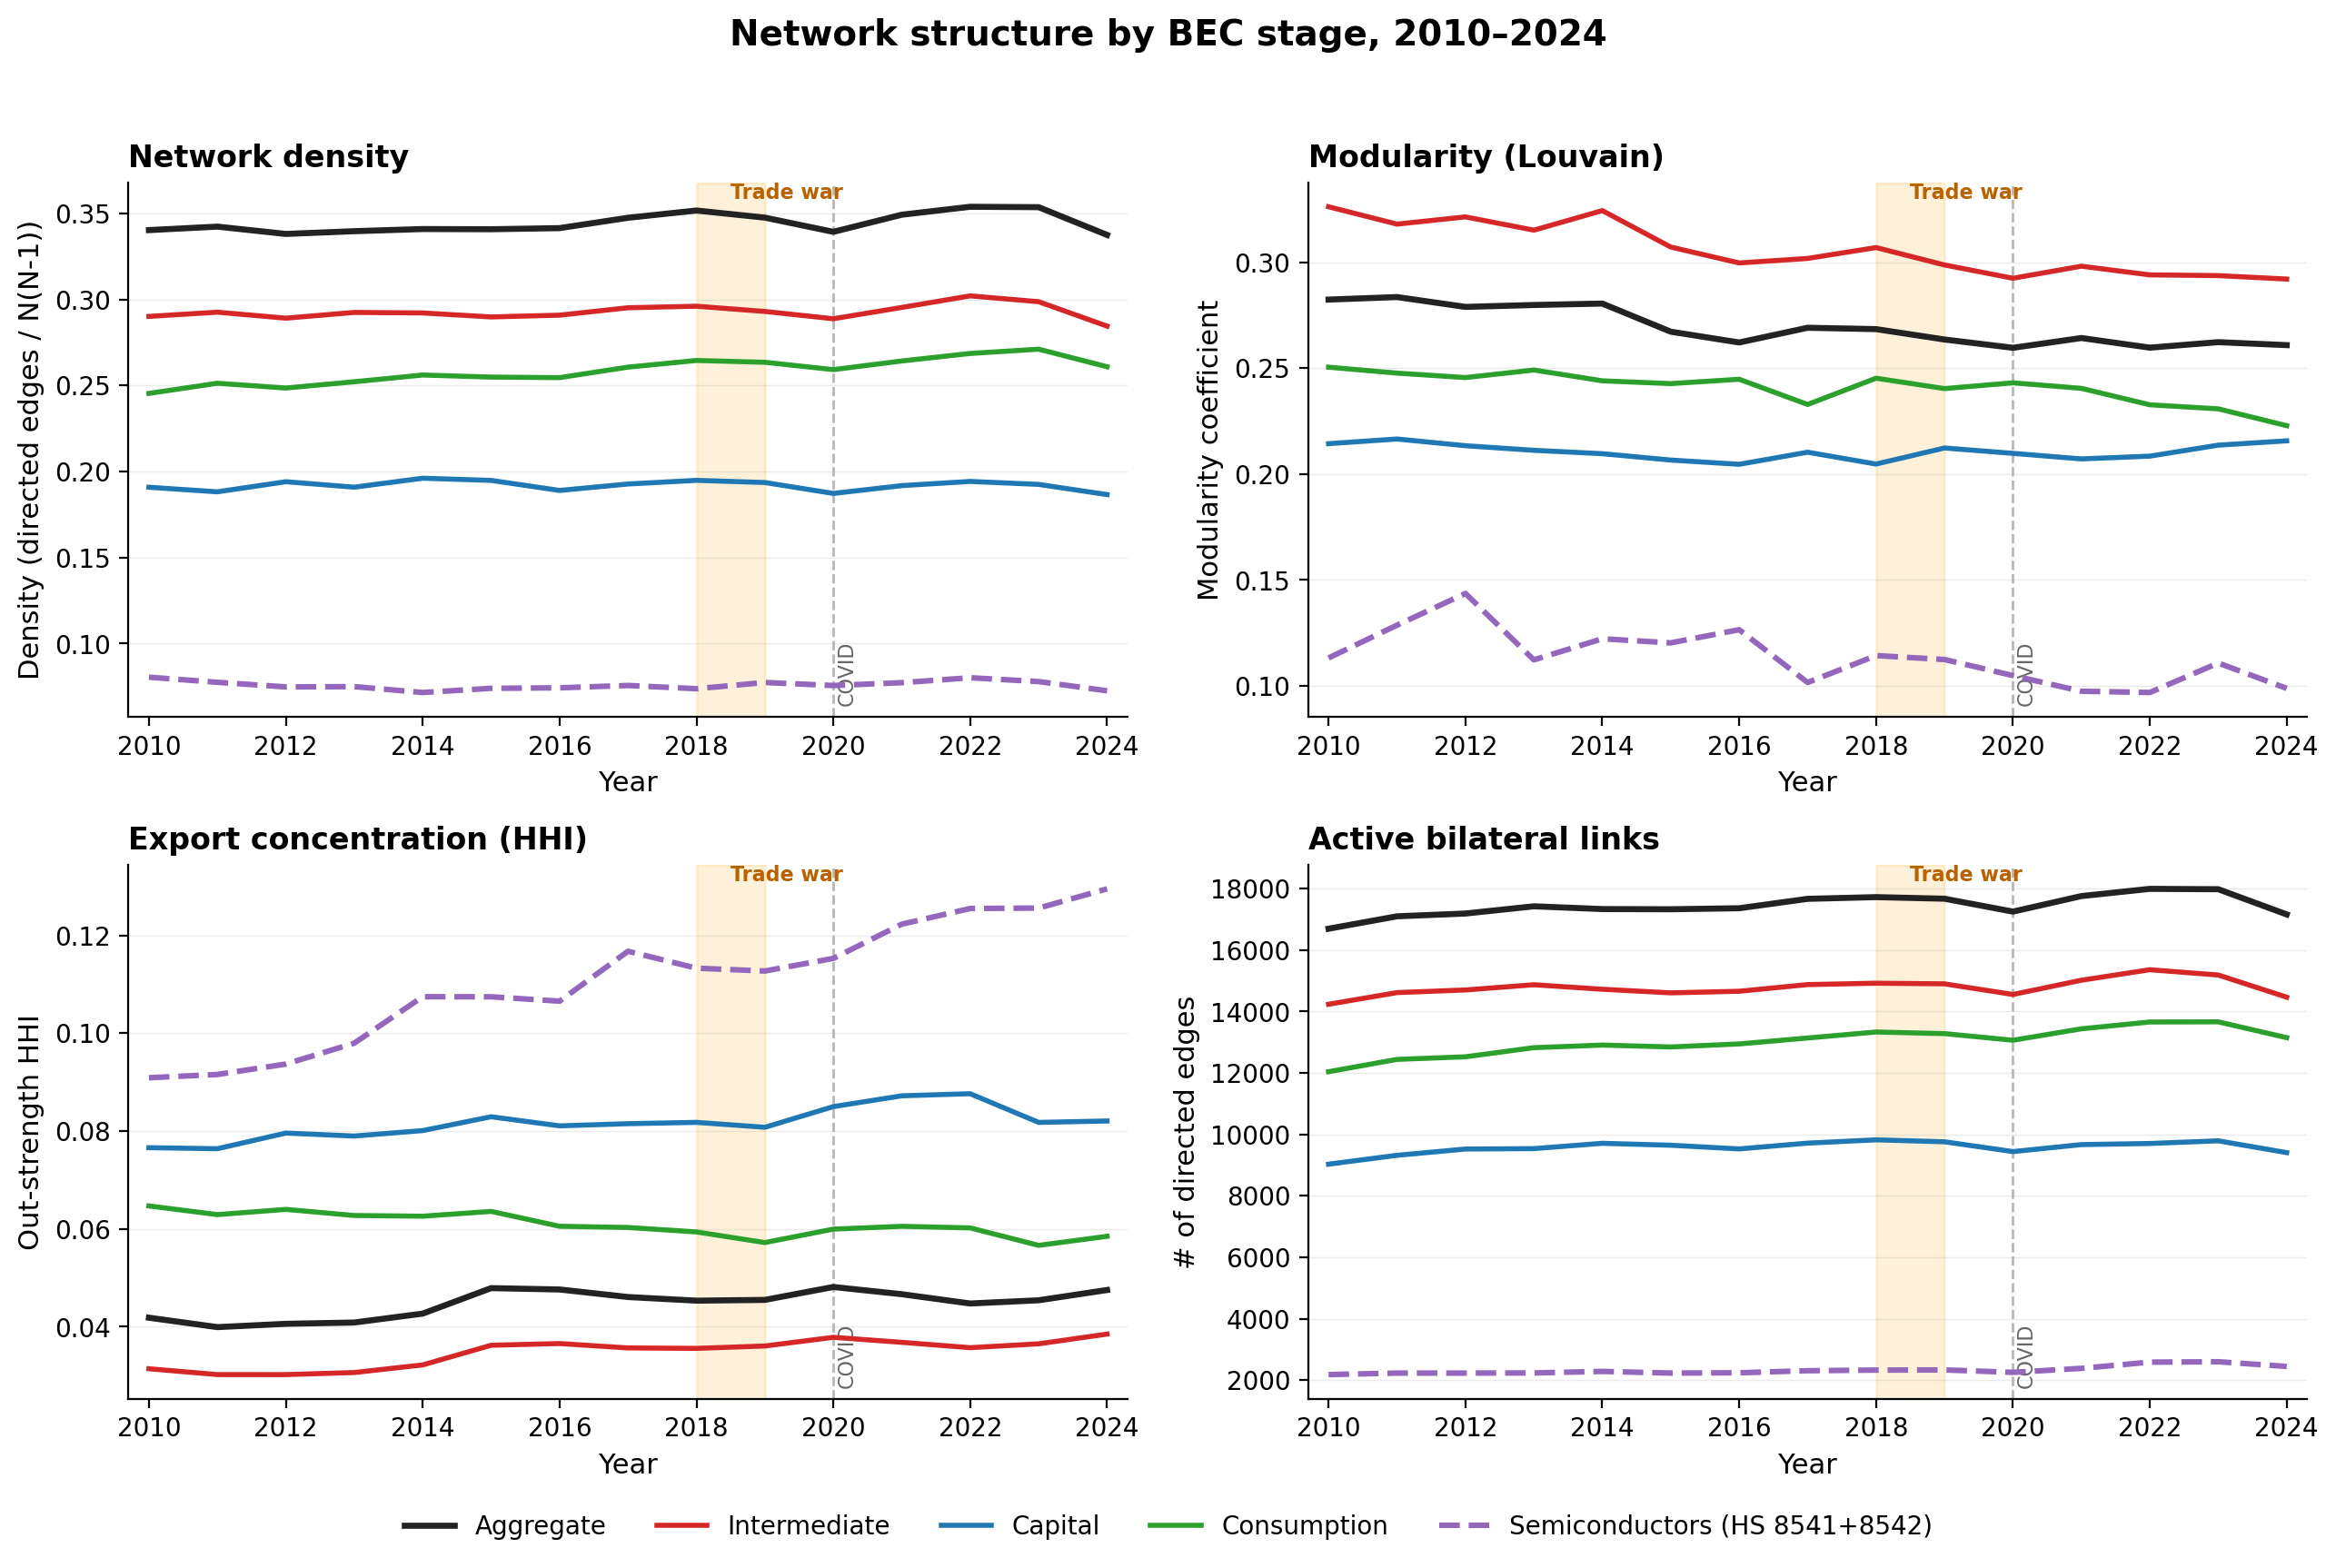
\includegraphics[width=\textwidth]{figures/fig1_network_metrics_levels.png}
  \caption{Network density, modularity, export concentration (HHI) and
  edge counts 2010--2024 for aggregate vs three BEC stages. Capital
  goods have dramatically higher HHI ($\sim$0.08) than the others
  ($\sim$0.04). Intermediate has the highest modularity throughout.}
  \label{fig:bec-levels}
\end{figure}

\begin{findbox}
\textbf{Modularity declined in intermediates and consumption}, was flat in
capital. This is contra-fragmentation: the GVC subnetwork (intermediates)
became more globally interconnected, not less, despite the trade war.

\textbf{Capital goods network is dramatically more concentrated} (HHI
$\sim$0.08 vs $\sim$0.04 for other stages). A handful of countries (CHN,
DEU, JPN, KOR, USA) dominate capital exports and that concentration is
stable or rising.

\textbf{China's dominance is stage-dependent.} In 2024 China's export share
of global trade is:
\begin{itemize}[leftmargin=*]
  \item Capital goods: \textbf{22.6\%}
  \item Consumption goods: 18.7\%
  \item Aggregate: 15.7\%
  \item Intermediates: \textbf{12.5\%}
\end{itemize}
Common framing about ``China dominating GVC intermediates'' is misleading.
China dominates capital goods. In intermediates it is both a major importer
\textit{and} exporter (typical hub behaviour).
\end{findbox}

\subsection{Vietnam's connector rise is intermediate-specific}

\begin{figure}[H]
  \centering
  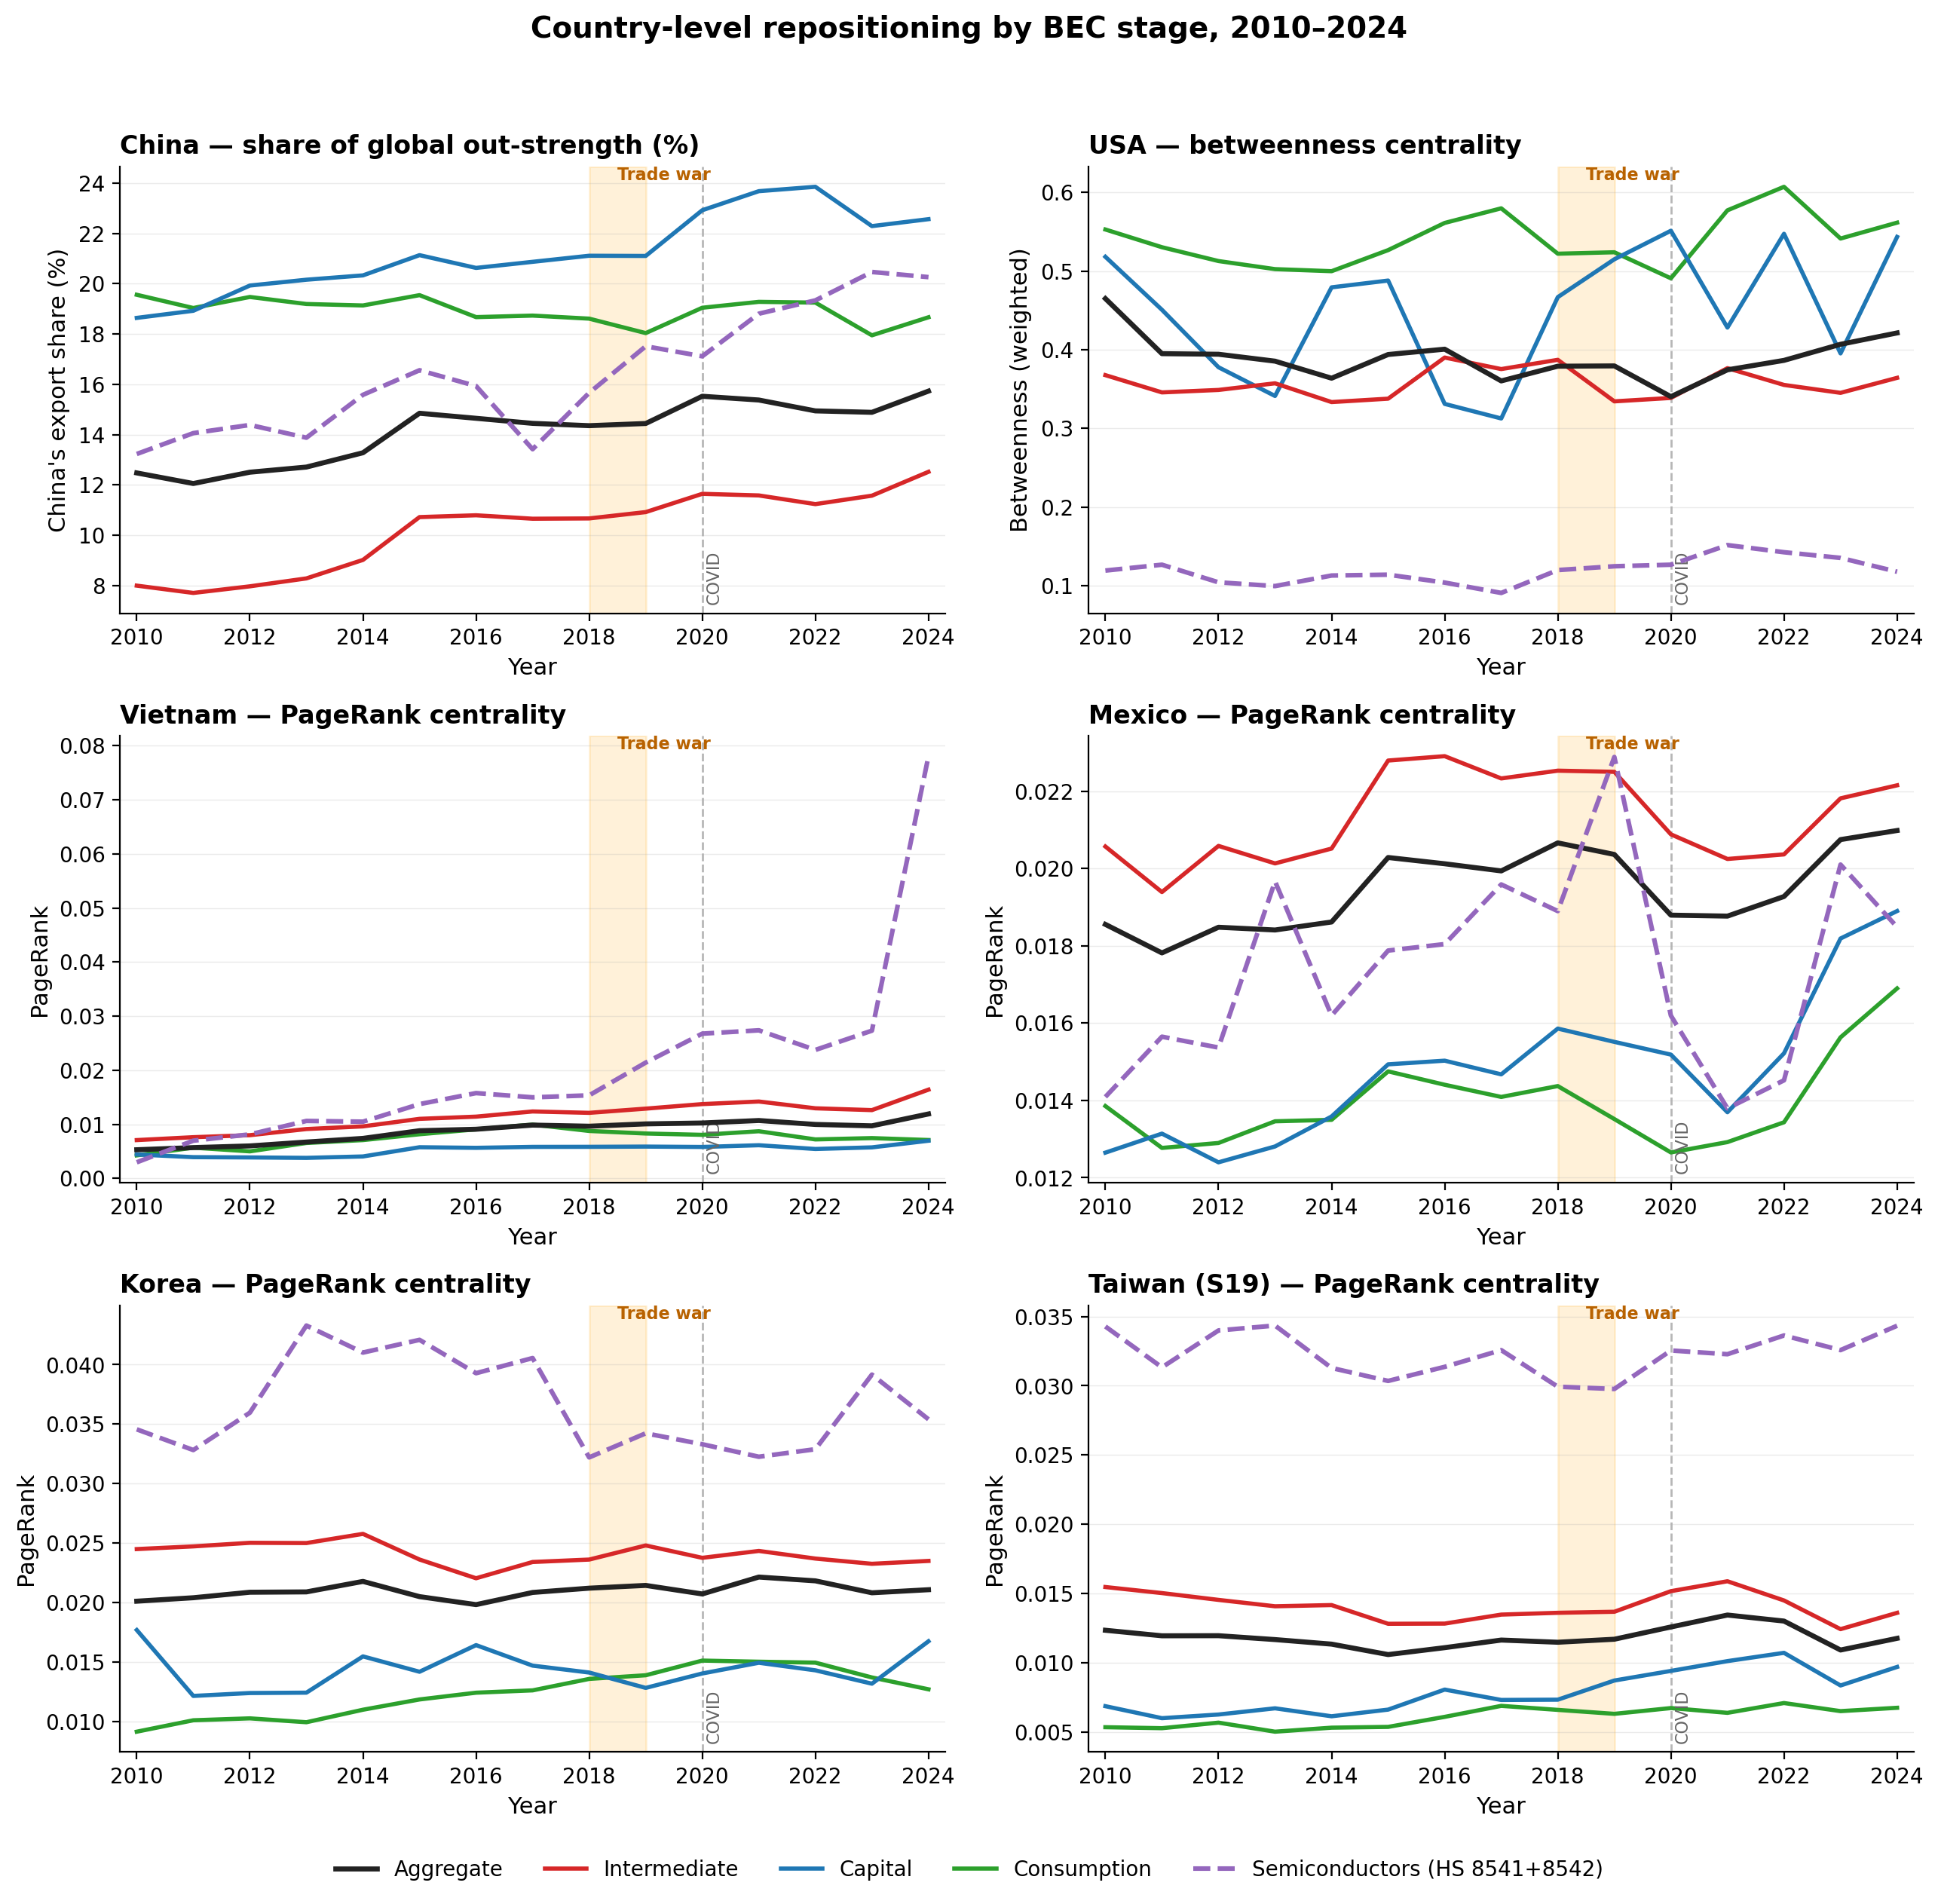
\includegraphics[width=\textwidth]{figures/fig3_country_panels.png}
  \caption{Country-level repositioning by BEC stage, 2010--2024. Vietnam's
  PageRank in intermediate goods (red) more than doubled; capital-goods
  PageRank (blue) stayed roughly flat. Vietnam's rise is specifically
  about intermediate-goods routing, not capital.}
  \label{fig:countries}
\end{figure}

% =====================================================================
\section{Phase B.3 — Semiconductor subnetwork}

PLAID's binary microchip indicator is too broad — it flags 100\% of HS4
chapters including washing machines, dishwashers, and bulldozers (because
they contain electronics). For a sharper analysis we use a direct HS6
filter: HS chapters \textbf{8541} (discrete semiconductors, LEDs,
photovoltaic) and \textbf{8542} (electronic integrated circuits). This
captures \$1.06~T of trade in 2023 (4.6\% of global trade), tightly
identified.

\begin{figure}[H]
  \centering
  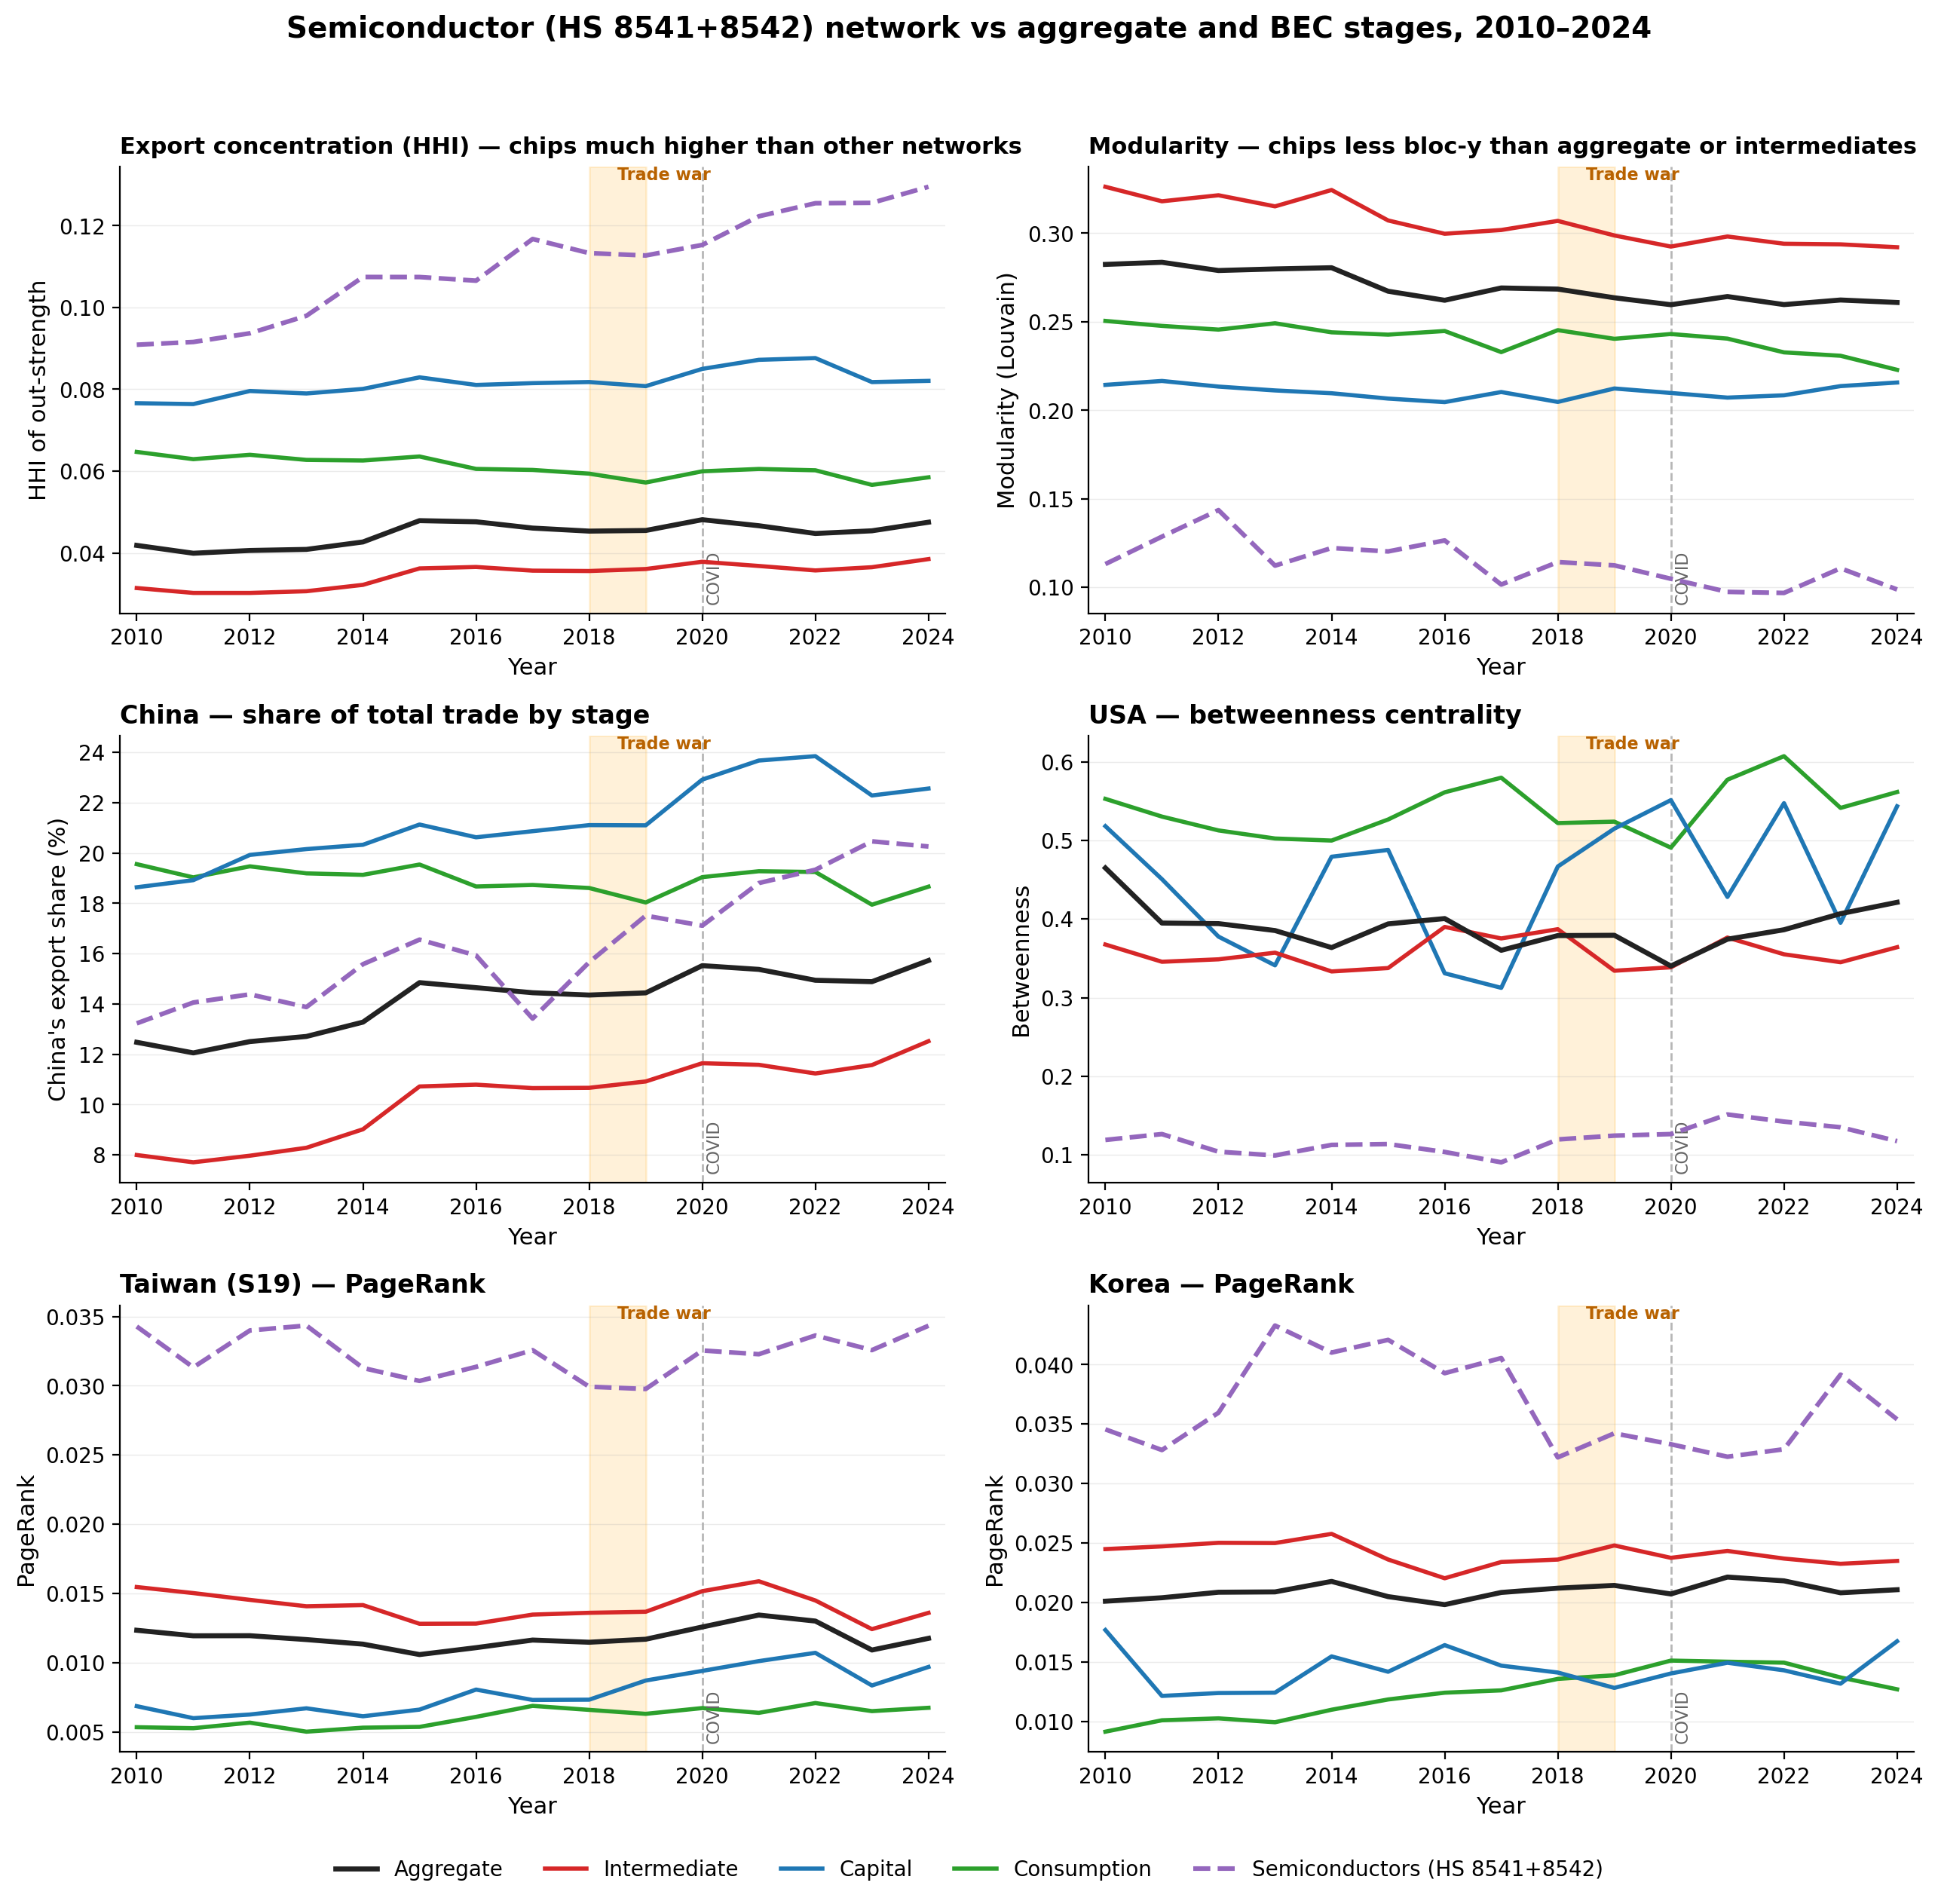
\includegraphics[width=\textwidth]{figures/fig5_semiconductors.png}
  \caption{Semiconductor (HS 8541+8542) network compared to aggregate
  and BEC stages, 2010--2024. The dashed purple line is semiconductors.}
  \label{fig:semi}
\end{figure}

\begin{findbox}
\textbf{Semiconductor network looks structurally different.}
HHI 0.13 in 2024 (3$\times$ higher than aggregate). Density 0.07 (vs 0.35
aggregate) — much sparser, hub-and-spoke. Modularity $\sim$0.10
(low) — \textit{not} bloc-structured but heavily hub-centric.

\textbf{Concentration rising over time.} HHI grew 0.084 (2005) $\to$ 0.130
(2024). Semiconductor production is consolidating, not diversifying.

\textbf{Taiwan dominates relative to its overall trade weight.} Taiwan's
aggregate global share is 2.5\%, but its semiconductor share is 21.4\% in
2024. Korea is next at 15.2\%.
\end{findbox}

\begin{limitbox}
HS 854140 mixes light-emitting diodes with photovoltaic (solar) panels.
China dominates solar; including it slightly inflates the
``semiconductor'' figure. For a stricter integrated-circuit-only analysis,
isolate HS 8542. The findings here are qualitatively the same in either case.
\end{limitbox}

% =====================================================================
\section{Phase C — The added value of stratification}

A key methodological argument for using the BEC and semiconductor
stratification is that the aggregate-trade view hides the country
specialisations that matter for the trade-war story. Figure~\ref{fig:heatmap}
makes this explicit.

\begin{figure}[H]
  \centering
  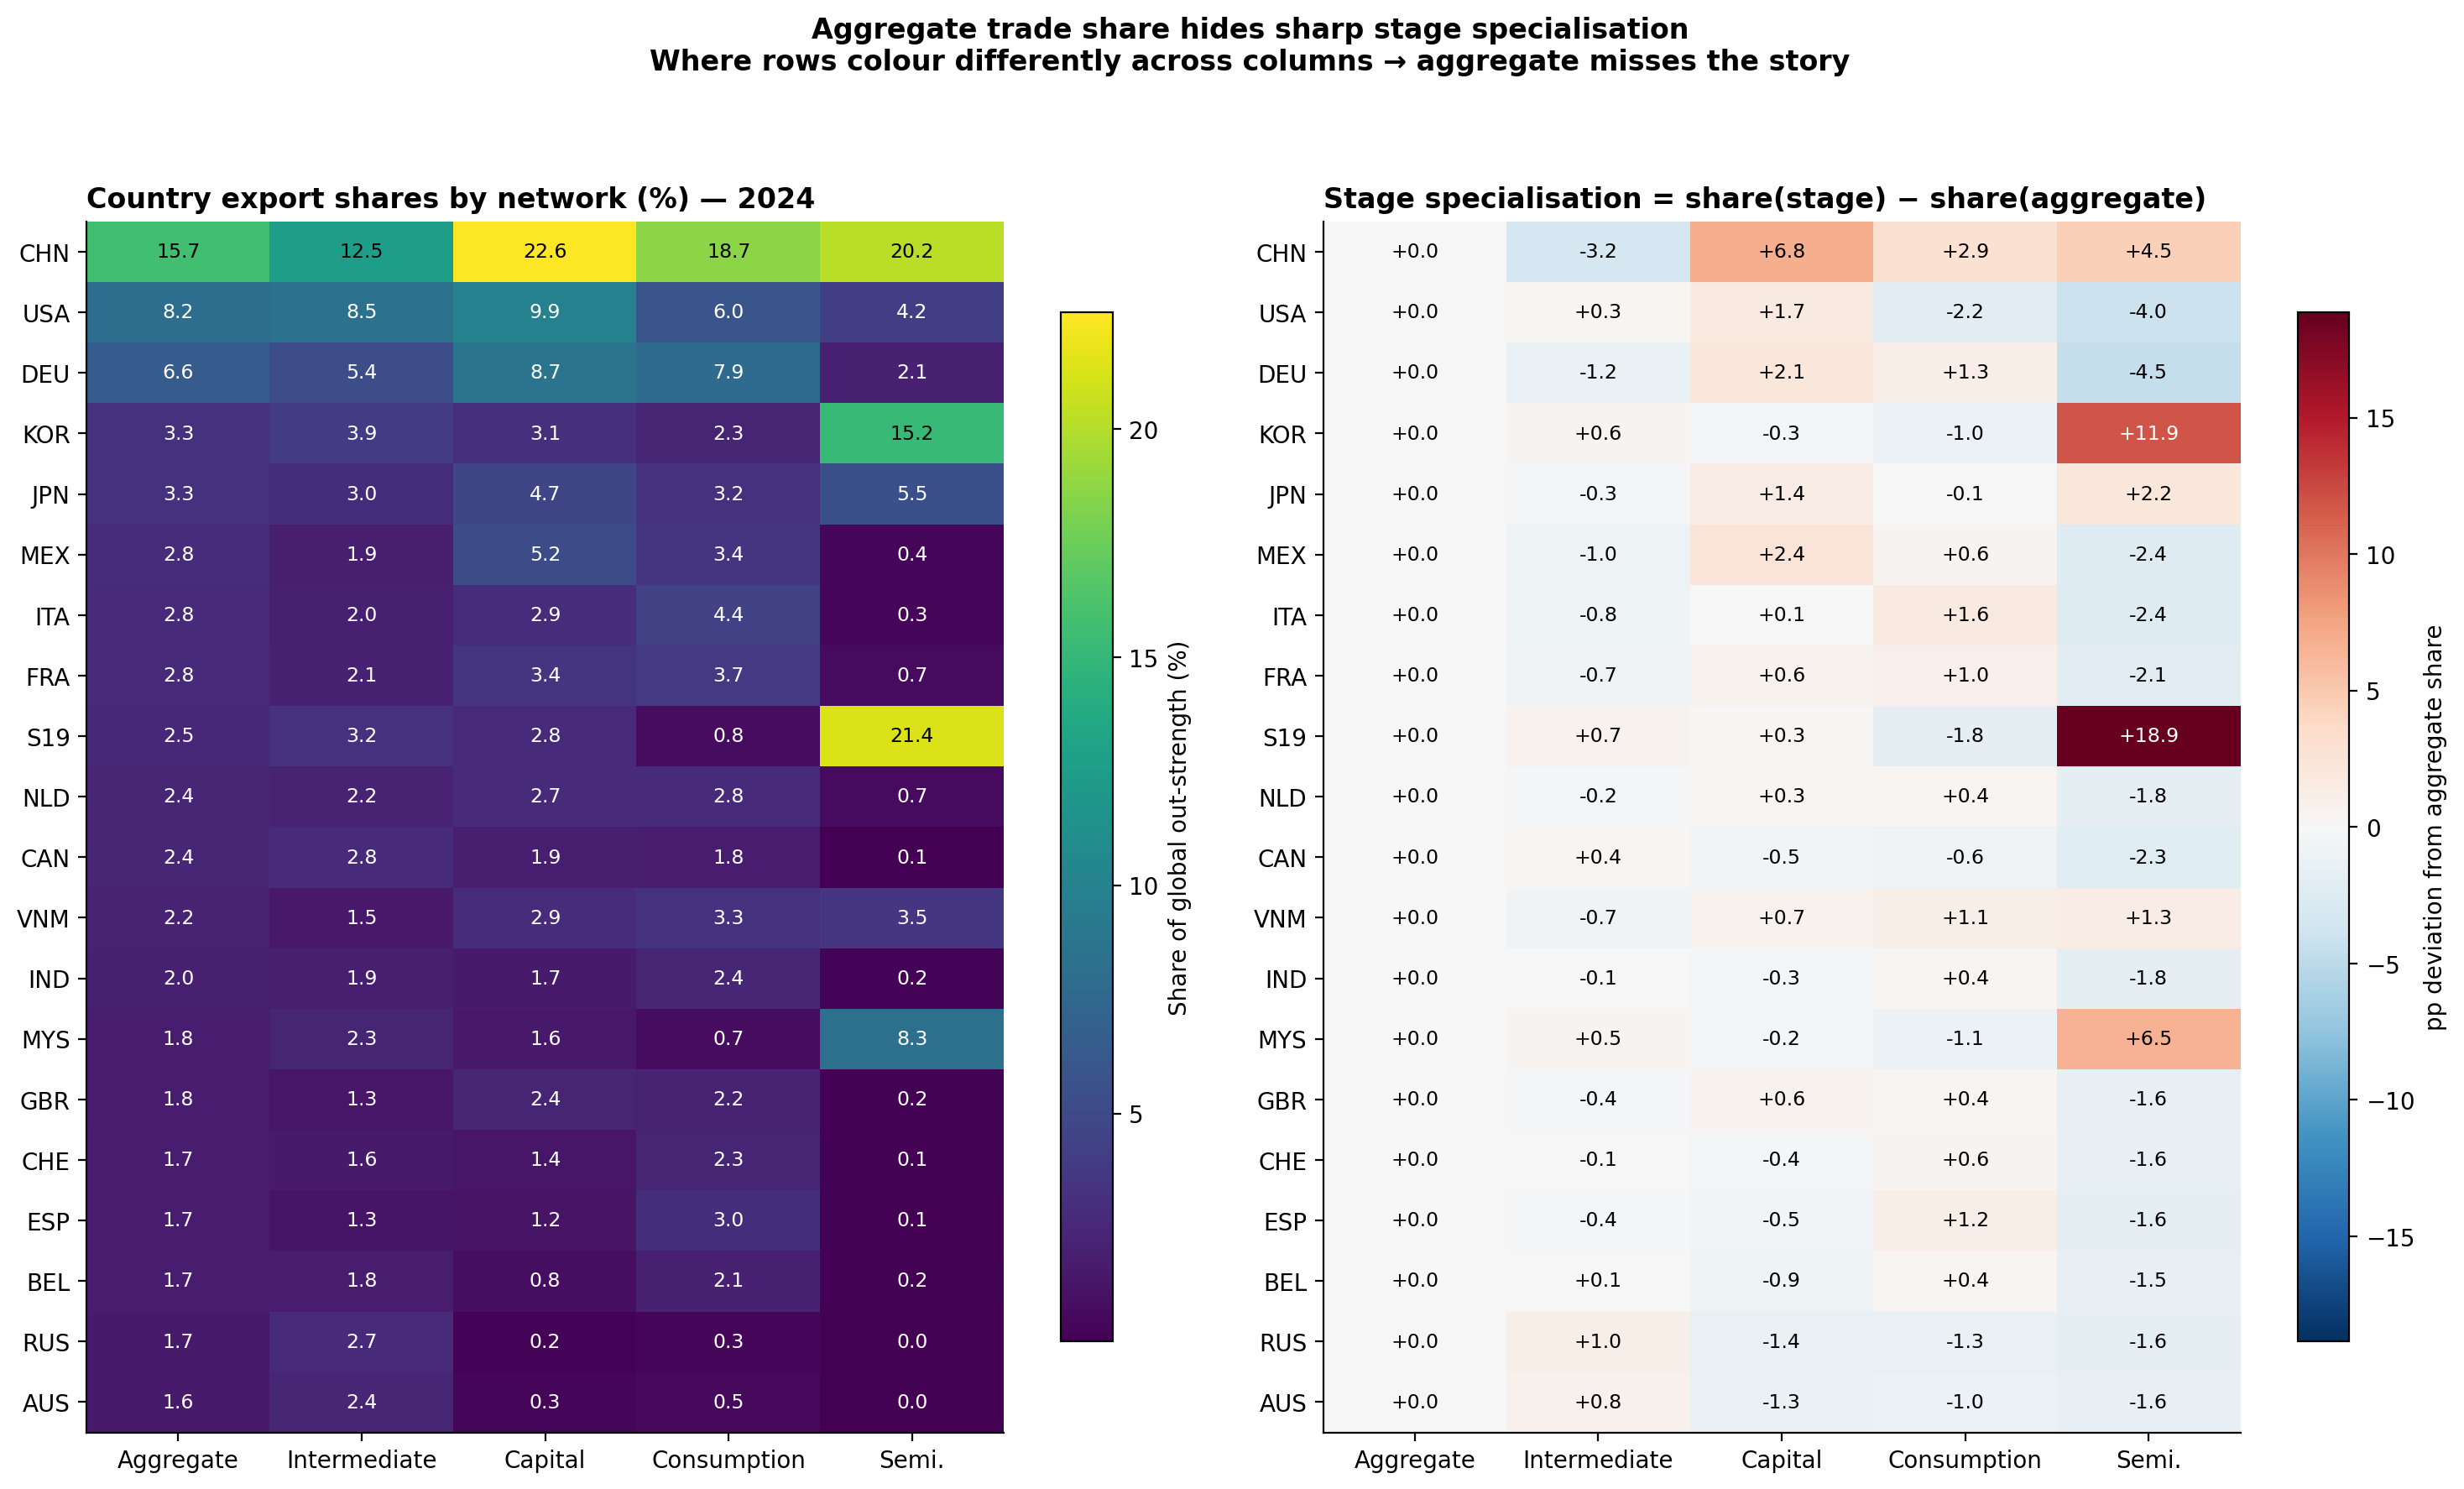
\includegraphics[width=\textwidth]{figures/fig7_specialization_heatmap.png}
  \caption{Country export shares by network in 2024. Left panel: levels.
  Right panel: deviation from the aggregate share (positive = country is
  over-represented in that stage). Where the row colour varies sharply
  across columns, the aggregate view is hiding the real story.}
  \label{fig:heatmap}
\end{figure}

\begin{findbox}
\textbf{Stratification reveals specialisations invisible in the aggregate}:
\begin{itemize}[leftmargin=*]
  \item Taiwan: aggregate 2.5\%, semiconductor 21.4\% — \textbf{+19.6 pp}
  \item Korea: aggregate 3.5\%, semiconductor 15.2\% — \textbf{+12.5 pp}
  \item Malaysia: aggregate 1.4\%, semiconductor 8.0\% — \textbf{+6.5 pp}
  \item China: aggregate 15.7\%, capital 22.6\% — \textbf{+6.9 pp};
        intermediate $-3.2$ pp
\end{itemize}
\textbf{Aggregate trade share is an unreliable proxy for stage-specific
position.}
\end{findbox}

\begin{limitbox}
A coloured-row label is still a partition of \textbf{gross} trade. Vietnam's
``consumption'' exports (e.g., laptops) embed intermediate value from Korea,
China and others. Distinguishing this requires the value-added decomposition
of input-output tables — which we do not perform here.
\end{limitbox}

% =====================================================================
\section{Phase D — Tariff-stratified networks}

After integrating the FGKK \texttt{z\_usch\_w} tariff data (US tariffs on
Chinese imports), we partition global bilateral trade by tariff treatment
status. The binary partition uses ``treated = HS6 in FGKK with
$z_{usch,w} > 0$''; a finer 4-bucket partition divides treated products by
post-tariff intensity (none / low 0--7.5\% / mid 7.5--17.5\% / high $>$17.5\%).

\subsection{Tariff facts}

\begin{itemize}[leftmargin=*]
  \item Of \$510B US imports from China in 2017,
        \textbf{59.4\% became tariffed} (post-trade-war).
  \item Tariff coverage by BEC stage:
        \textbf{intermediates 78.9\%} treated (avg weighted tariff
        \textbf{8.60\%}), consumption 65.2\% (3.95\%),
        \textbf{capital only 29.5\%} (3.57\%).
  \item Semiconductors (HS 8541+8542): all 13 covered HS6 codes treated.
        \textbf{Real integrated circuits (8542) got only 5.7--8.9\%}
        tariffs; LEDs/solar (854140) hit 25.2\%.
\end{itemize}

\begin{findbox}
\textbf{The most aggressively tariffed stage was intermediates, not
capital.} Capital goods — where China actually dominates — were the
\textit{least} tariffed. This explains why our network analysis shows
China's capital-goods centrality continued to rise after 2018: there was
no policy pressure to substitute it.
\end{findbox}

\subsection{The puzzle: China's global share rose in highly tariffed products}

We ran the long-run pipeline on each tariff bucket
(\texttt{long\_run\_metrics\_tariff.py}) and looked at China's export
share by stratum.

\begin{figure}[H]
  \centering
  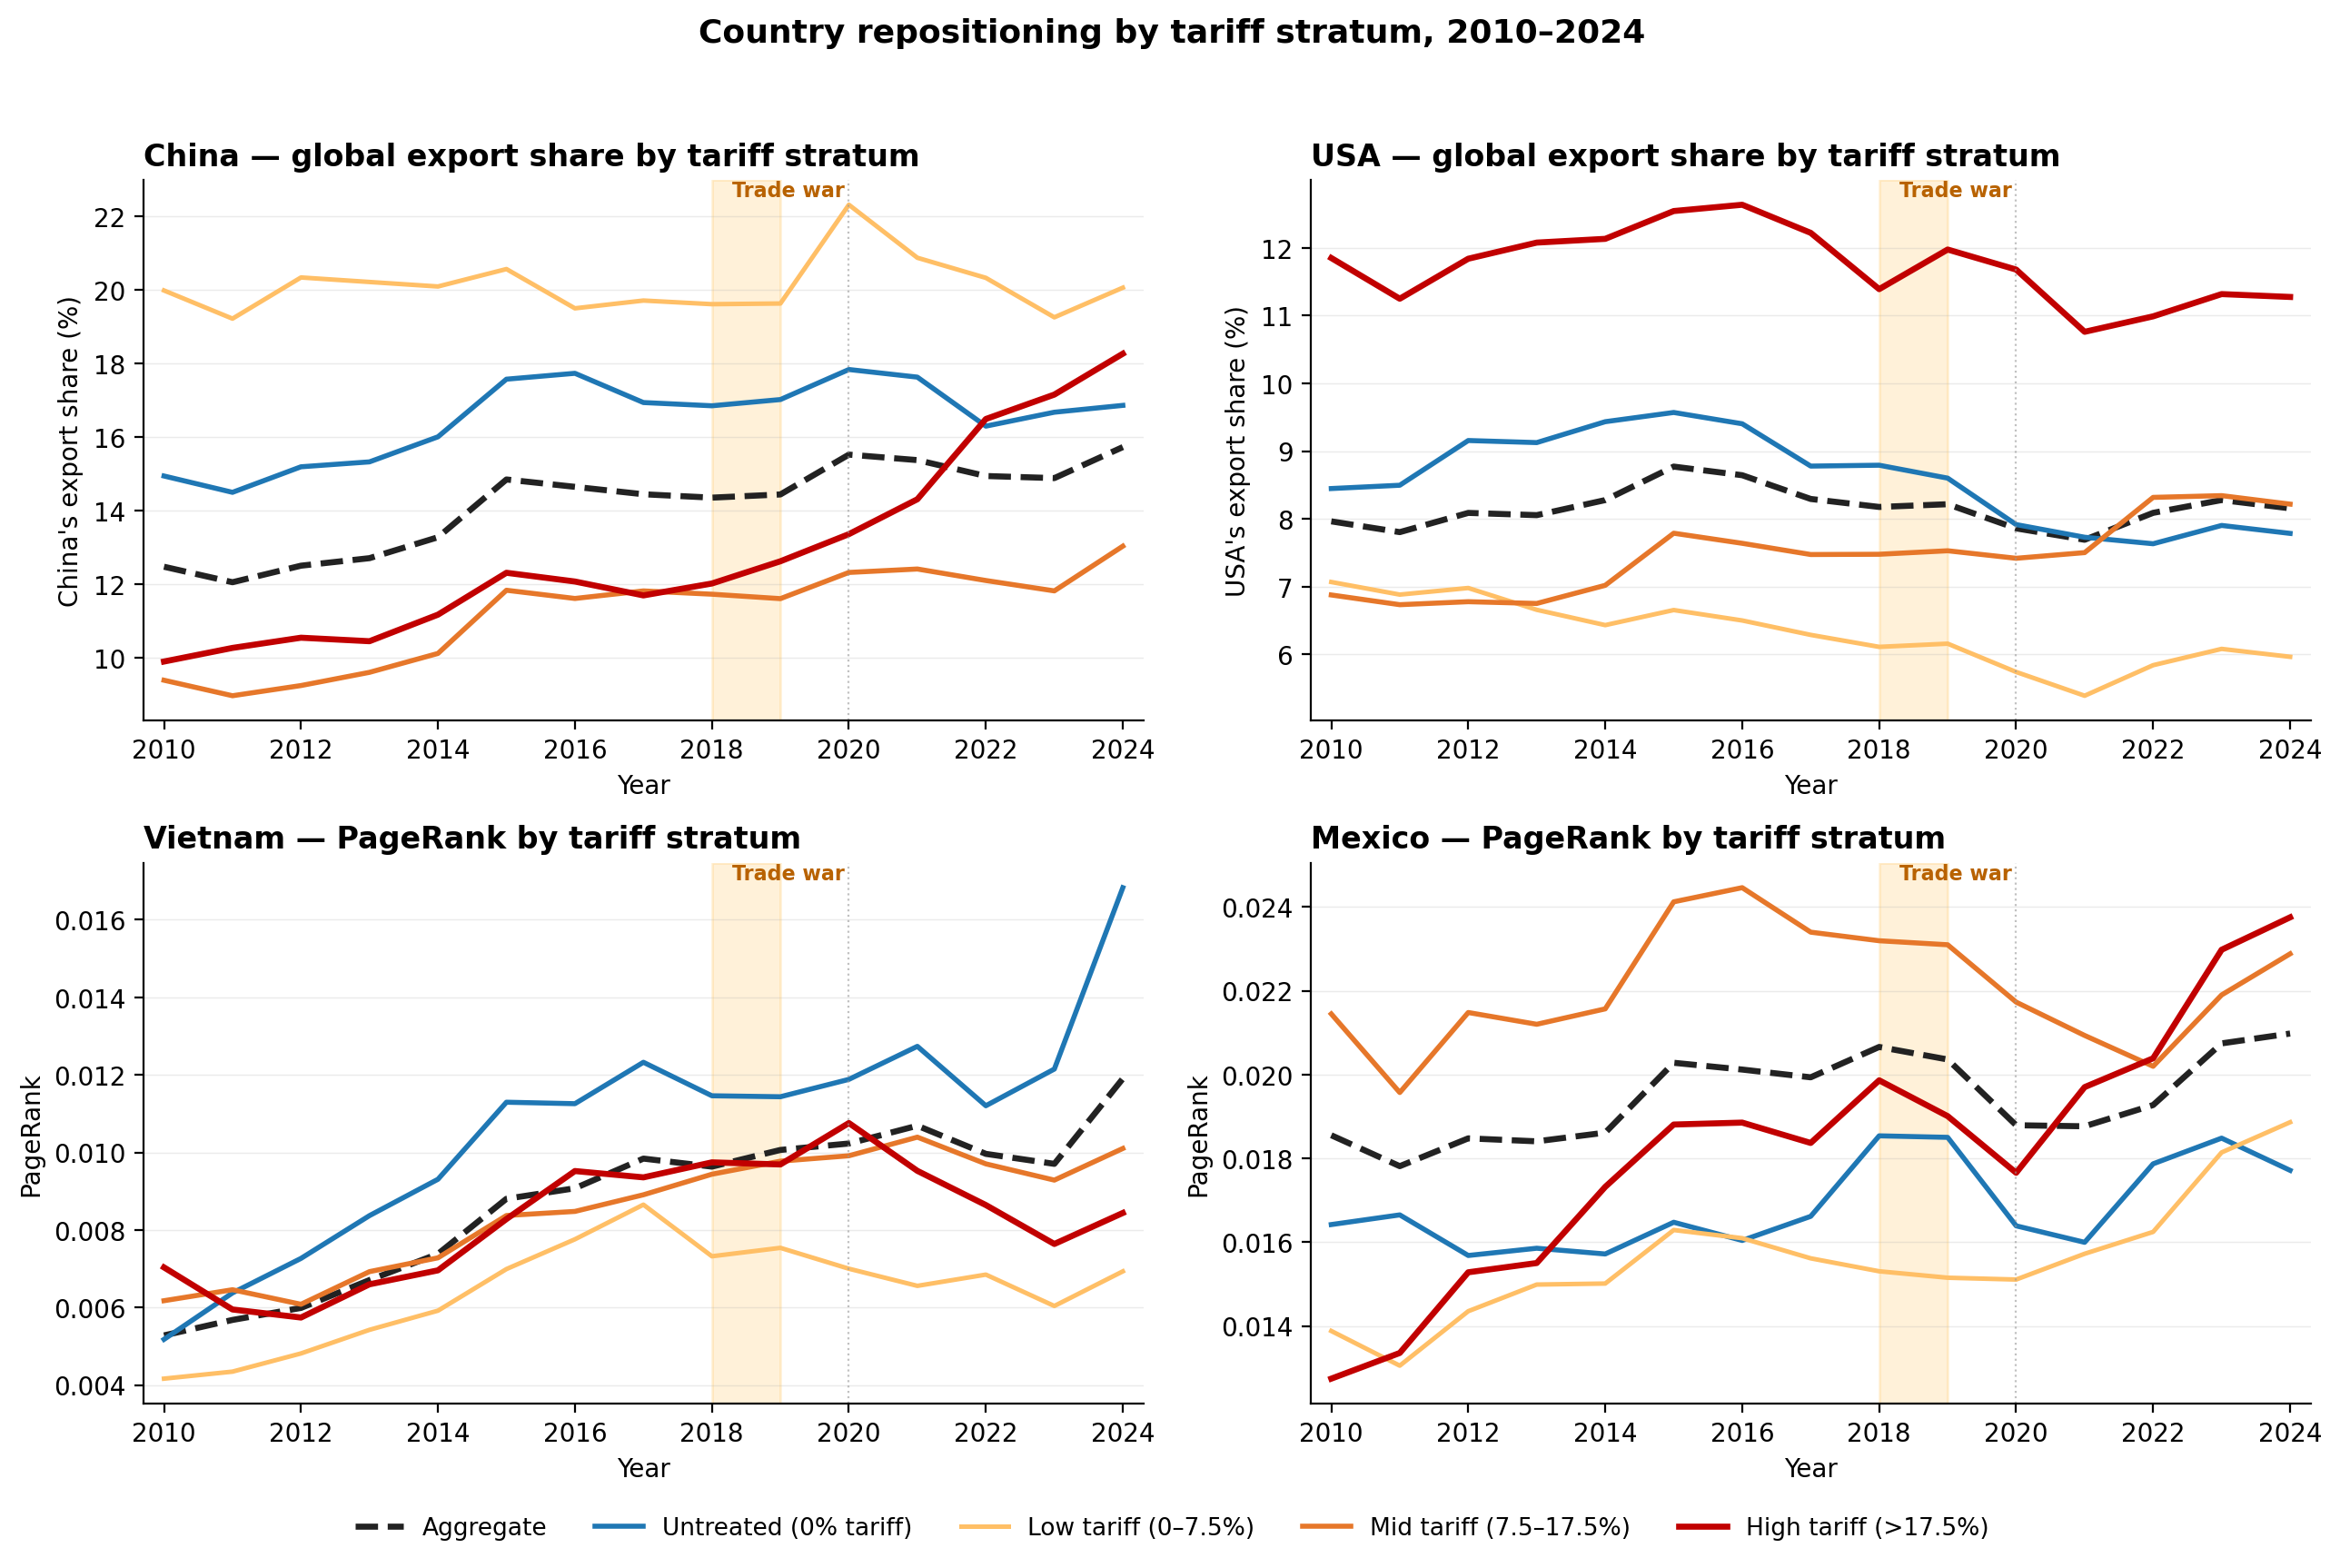
\includegraphics[width=\textwidth]{figures/fig10_tariff_country_panels.png}
  \caption{Country repositioning by tariff stratum, 2010--2024. China's
  share \textit{rose} in high-tariff products globally. Mexico rose
  more in tariffed products; Vietnam rose in untariffed.}
  \label{fig:tariff-countries}
\end{figure}

\begin{findbox}
\textbf{Counter-intuitive finding}: In products that USA tariffed most
heavily ($>$17.5\%), China's \textit{global} export share grew from 11.7\%
(2017) to \textbf{18.3\%} (2024) — a 6.6~pp increase.

This is not a diversion failure. It is \textit{displacement}: USA tariffs
collapsed Chinese exports to the USA in these products, but China redirected
those exports to non-US markets (EU, ASEAN, LatAm, Africa) and gained share
there. The global-network view captures this redirection rather than the
US-side diversion.

This is precisely why the next phase isolates US-as-importer flows: the
global view masks the actual diversion story.
\end{findbox}

\begin{limitbox}
The global tariff-stratification view aggregates global trade in tariffed
products. It cannot separate \textit{US imports from China shifting away}
from \textit{Chinese exports being redirected to non-US destinations}. The
narrative ``the trade war shifted China's global share'' is a mixture of
these two mechanisms and the two cannot be untangled at this level.
\end{limitbox}

% =====================================================================
\section{Phase E — Friend-shoring analysis at HS6 level}

To isolate the bilateral diversion story, we filter BACI to
\textbf{USA as importer only}, look at the HS6 codes flagged as tariffed
under FGKK, and decompose the source-country mix over time. To distinguish
genuine production relocation from transshipment, we additionally inspect
each connector country's mix of intermediate imports — the hypothesis is:

\begin{itemize}[leftmargin=*]
  \item \textbf{Transshipment-flavoured}: connector's exports to USA rise
        \textit{and} China's intermediate exports to the connector rise.
        Same Chinese inputs, new shipping address.
  \item \textbf{Relocation-flavoured}: connector's exports to USA rise
        \textit{but} China's intermediate share of the connector's
        intermediate imports falls (or stays flat) while non-Chinese
        sources rise. Connector building genuine local production
        capacity using non-Chinese inputs.
\end{itemize}

\subsection{US imports of tariffed products}

\begin{figure}[H]
  \centering
  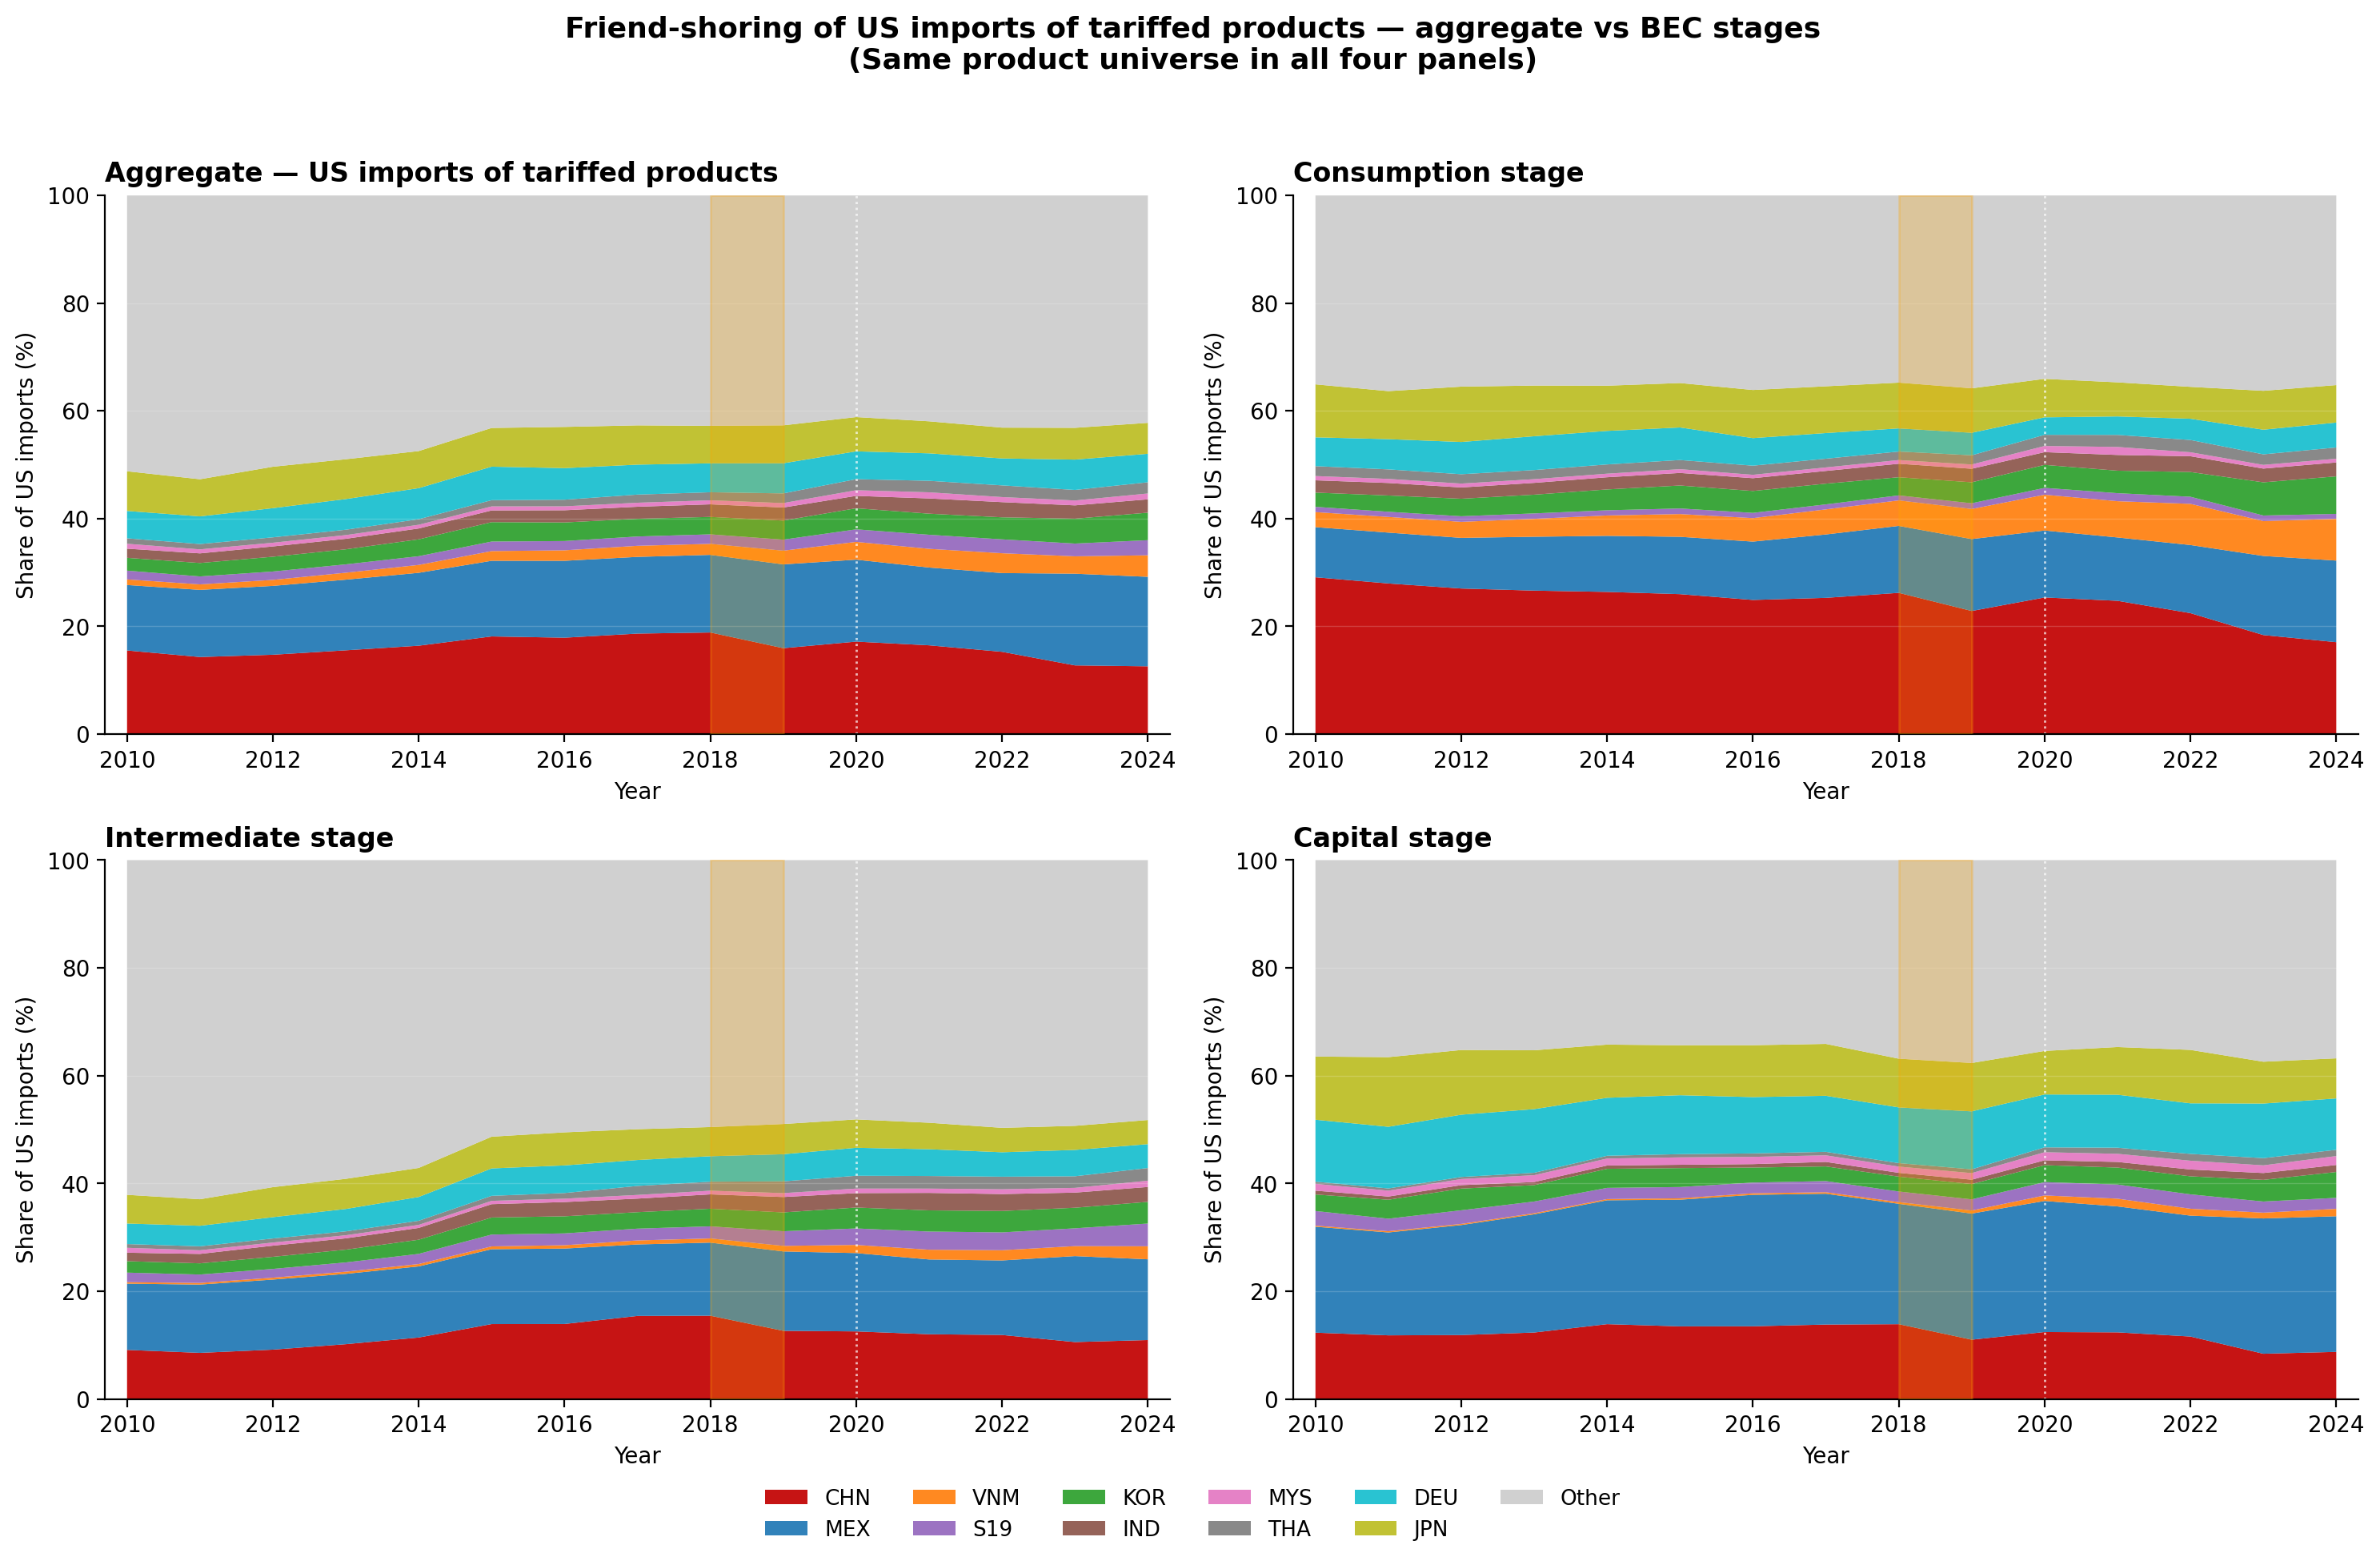
\includegraphics[width=\textwidth]{figures/fig11_friendshoring_aggregate_vs_bec.png}
  \caption{US imports of tariffed products, by source country and BEC stage,
  2010--2024. Same product universe in all four panels.}
  \label{fig:fs}
\end{figure}

\begin{findbox}
\textbf{China lost \$24~B and 6.1 percentage points of US import share}
in tariffed products 2017$\to$2024 (aggregate view). The diversion is
\textbf{sharpest in consumption goods} ($-8.2$~pp) and least sharp in
intermediates ($-4.5$~pp). In dollar terms, China's intermediate exports
to the USA fell only \$3~B — its share declined mostly because the market
grew.

\textbf{Winners}:
\begin{itemize}[leftmargin=*]
  \item \textbf{Mexico}: $+\$125$~B, +2.4 pp; dominant in capital
        goods (25\% share, stable).
  \item \textbf{Korea}: $+\$55$~B, +1.8 pp; largest gain in
        capital ($+171\%$ dollar growth in capital) and consumer goods.
  \item \textbf{Vietnam}: $+\$51$~B, +1.9 pp; biggest \%
        growth ($+163\%$). Particularly in consumer ($+\$27$~B) and
        intermediate ($+\$20$~B; $+346\%$).
  \item \textbf{Taiwan}: $+\$31$~B; intermediate-only ($+164\%$,
        the semiconductor story).
\end{itemize}
\textbf{Losers}: Japan ($-1.6$ pp aggregate, $-2.2$ pp in capital),
Germany ($-0.3$ pp aggregate, $-0.9$ pp in capital).
\end{findbox}

\subsection{Connectors' intermediate-import source mix —
the transshipment vs relocation discriminator}

\begin{figure}[H]
  \centering
  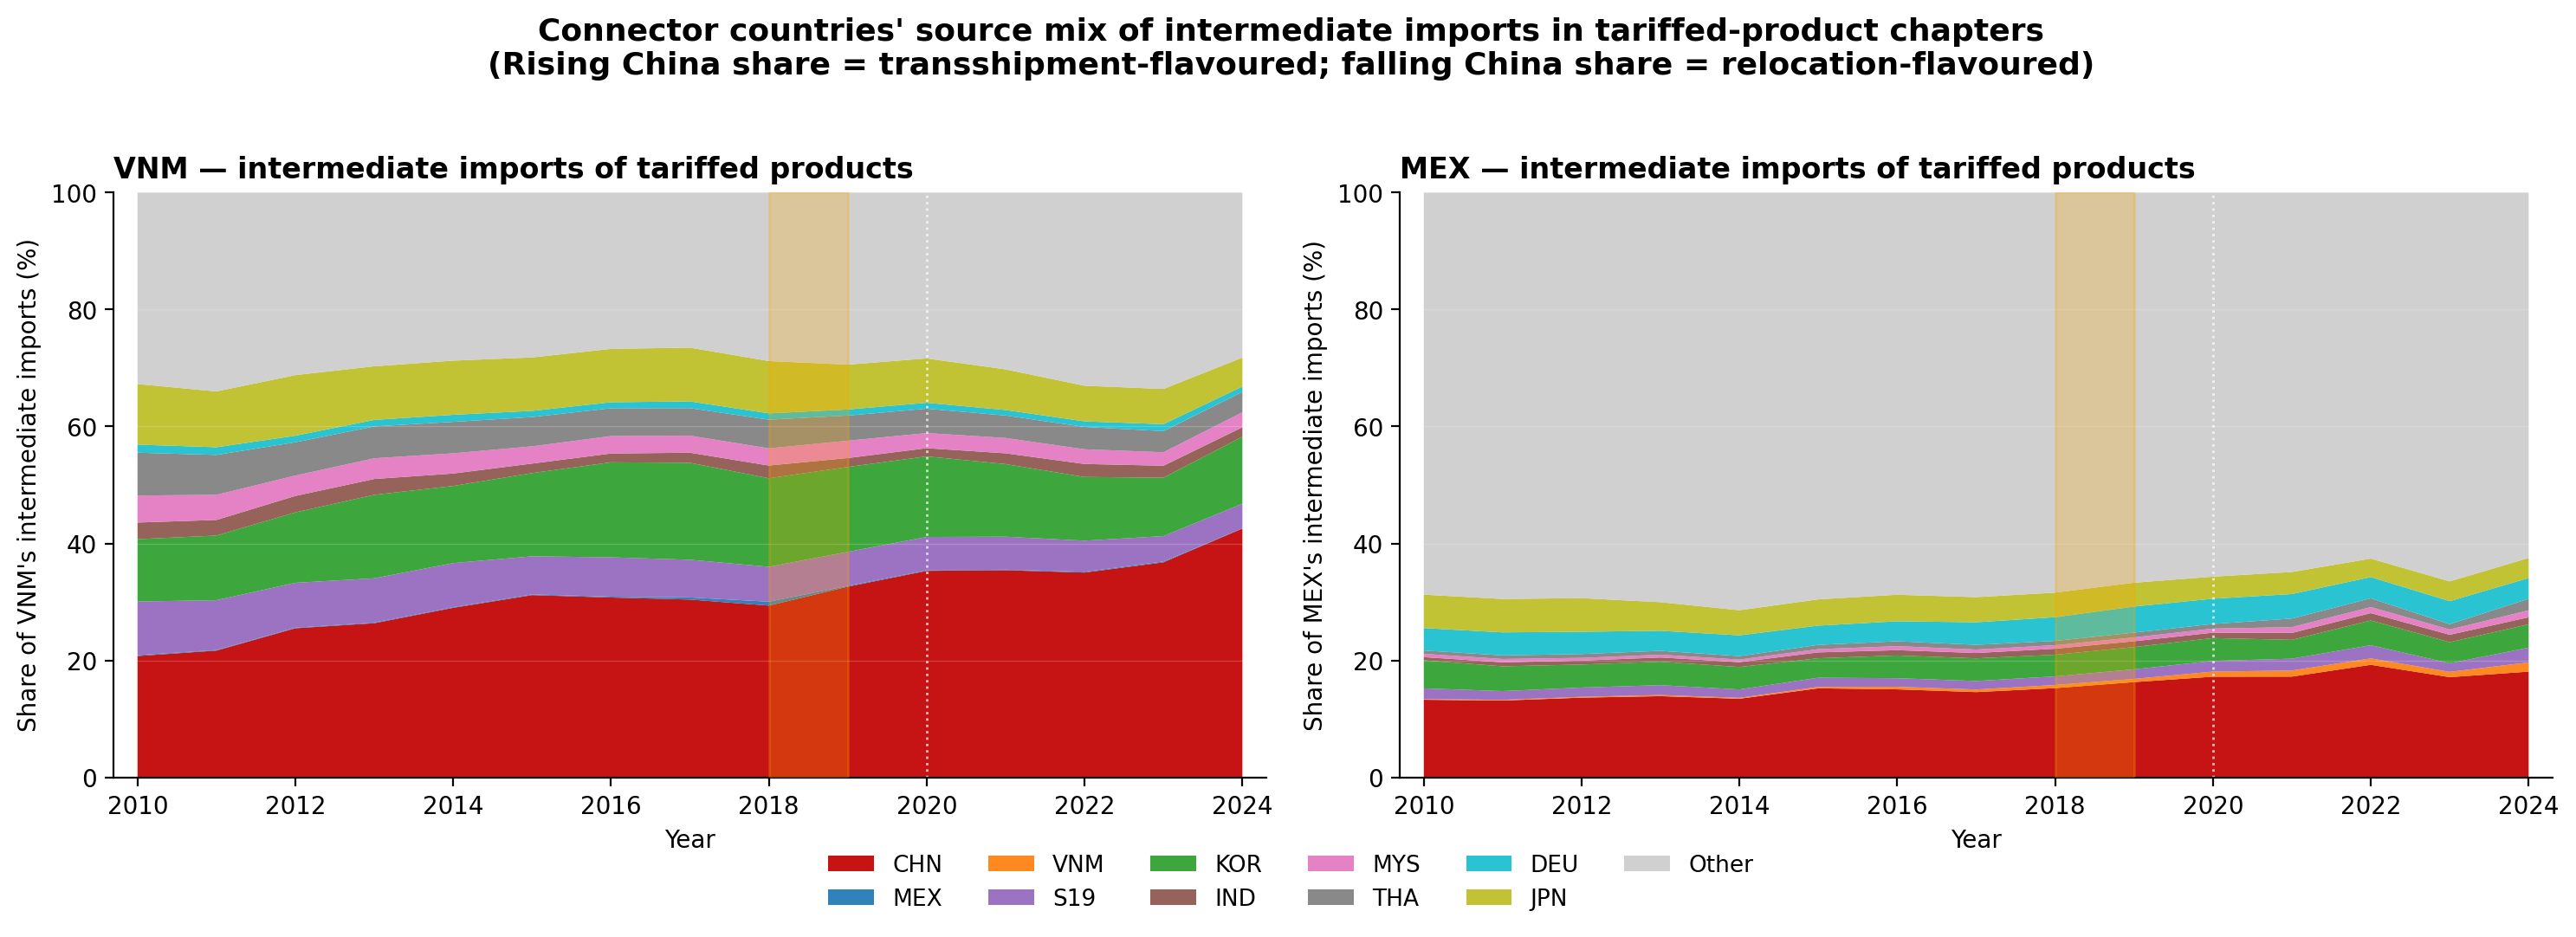
\includegraphics[width=\textwidth]{figures/fig12_connector_intermediate_source_mix.png}
  \caption{Vietnam and Mexico: source-country share of their intermediate
  imports of tariffed products, 2010--2024. Rising China share is a
  transshipment-flavoured signature.}
  \label{fig:connector}
\end{figure}

\begin{findbox}
\textbf{Vietnam looks transshipment-flavoured.} China's share of Vietnam's
intermediate imports in tariffed-product chapters grew from \textbf{30.4\%
(2017) to 42.6\% (2024)} — a 12 percentage point jump. As Vietnam ships
more to USA, it sources more inputs from China.

\textbf{Mexico looks more relocation-flavoured.} China's share of Mexico's
intermediate imports rose only modestly (14.6\% $\to$ 18.1\%, $+3.5$ pp).
Mexico's intermediate base remains US- and EU-anchored, with broader
diversification rather than concentration on China.

These are not statements about value-added (which we cannot observe), but
the gross-trade pattern is consistent with the two different mechanisms.
\end{findbox}

\subsection{Tabular summary}

The headline numbers are reported in Table~\ref{tab:fs} for the aggregate
view. Full tables (per-stage and connector-source-mix) are saved as
\texttt{tables/friendshoring\_us\_imports.csv} and
\texttt{tables/friendshoring\_connector\_sources.csv}.

\begin{table}[H]
\centering
\small
\caption{US imports of tariffed products: source-country shares and values,
2017 vs 2024 (aggregate, no BEC stratification).}
\label{tab:fs}
\begin{tabular}{lrrrrr}
\toprule
Source & Share 2017 & Share 2024 & $\Delta$ pp & $\Delta$ \$B & $\Delta$ \% \\
\midrule
CHN & 18.7\% & 12.6\% & $-6.07$ & $-24.3$ & $-8.6$ \\
MEX & 14.2\% & 16.6\% & $+2.37$ & $+125.5$ & $+58.1$ \\
VNM & 2.1\% & 4.0\% & $+1.94$ & $+51.0$ & $+163.3$ \\
KOR & 3.3\% & 5.1\% & $+1.82$ & $+55.1$ & $+110.3$ \\
S19 (Taiwan) & 1.7\% & 2.8\% & $+1.08$ & $+31.4$ & $+119.7$ \\
THA & 1.5\% & 2.1\% & $+0.57$ & $+19.8$ & $+86.2$ \\
CAN & 14.4\% & 14.9\% & $+0.56$ & $+89.0$ & $+40.8$ \\
DEU & 5.6\% & 5.3\% & $-0.27$ & $+24.3$ & $+28.9$ \\
JPN & 7.3\% & 5.7\% & $-1.55$ & $+7.5$ & $+6.8$ \\
\bottomrule
\end{tabular}
\end{table}

\begin{limitbox}
\textbf{Still circumstantial, not value-added decomposition.} We can't say
``X\% of Vietnam's exports to USA are passthrough Chinese value-added.''
That requires TiVA/ICIO.

\textbf{Tariff dummy is binary} ($z_{usch,w} > 0$). The same exercise on
high-tariff-only products ($>17.5\%$) would sharpen the diversion signal.

\textbf{No HS6$\to$HS6 product linkage.} We cannot trace specific Chinese
chip $X$ into specific Vietnamese laptop $Y$. The transshipment vs
relocation reading is at the country-chapter aggregate, not at the
product-input level.
\end{limitbox}

% =====================================================================
\section{Phase F — Network resilience analysis}

The first six phases established \textit{what} restructured. Resilience
analysis asks \textit{how robust} the network is to disruption — and
whether the trade war shifted that profile. This uses genuine
network-theoretic concepts that flow / share analysis cannot deliver.

\subsection{Network resilience glossary}

\begin{glossbox}{Resilience terms}
\textbf{Algebraic connectivity ($\lambda_2$)}: the second-smallest eigenvalue
of the graph Laplacian. Higher = harder to disconnect the graph by removing
edges. A theoretical scalar measure of structural robustness (Fiedler 1973).

\textbf{k-core decomposition}: iteratively peel off all nodes of degree $<k$.
The innermost surviving subgraph is the ``k-shell.'' Track the
\textit{max k} over time: rising = the dense backbone is getting deeper.

\textbf{Bridge edge}: an edge whose removal disconnects the graph (or
fragments it). Typically a periphery-to-core link; the country at the
periphery is only connected through that single link.

\textbf{Targeted-attack robustness}: simulate removing top-$k$ countries by
out-strength (or other centrality). Measure how quickly the largest
connected component shrinks. Curves that drop faster = more vulnerable
to losing hub countries.

\textbf{Disparity-filter backbone} (Serrano, Bogu\~n\'a, Vespignani 2009):
keep only edges that are statistically significant given each node's
weight distribution. Strips out noise; reveals the load-bearing skeleton.
\end{glossbox}

\subsection{Aggregate resilience (\texttt{resilience\_aggregate.py})}

\begin{figure}[H]
  \centering
  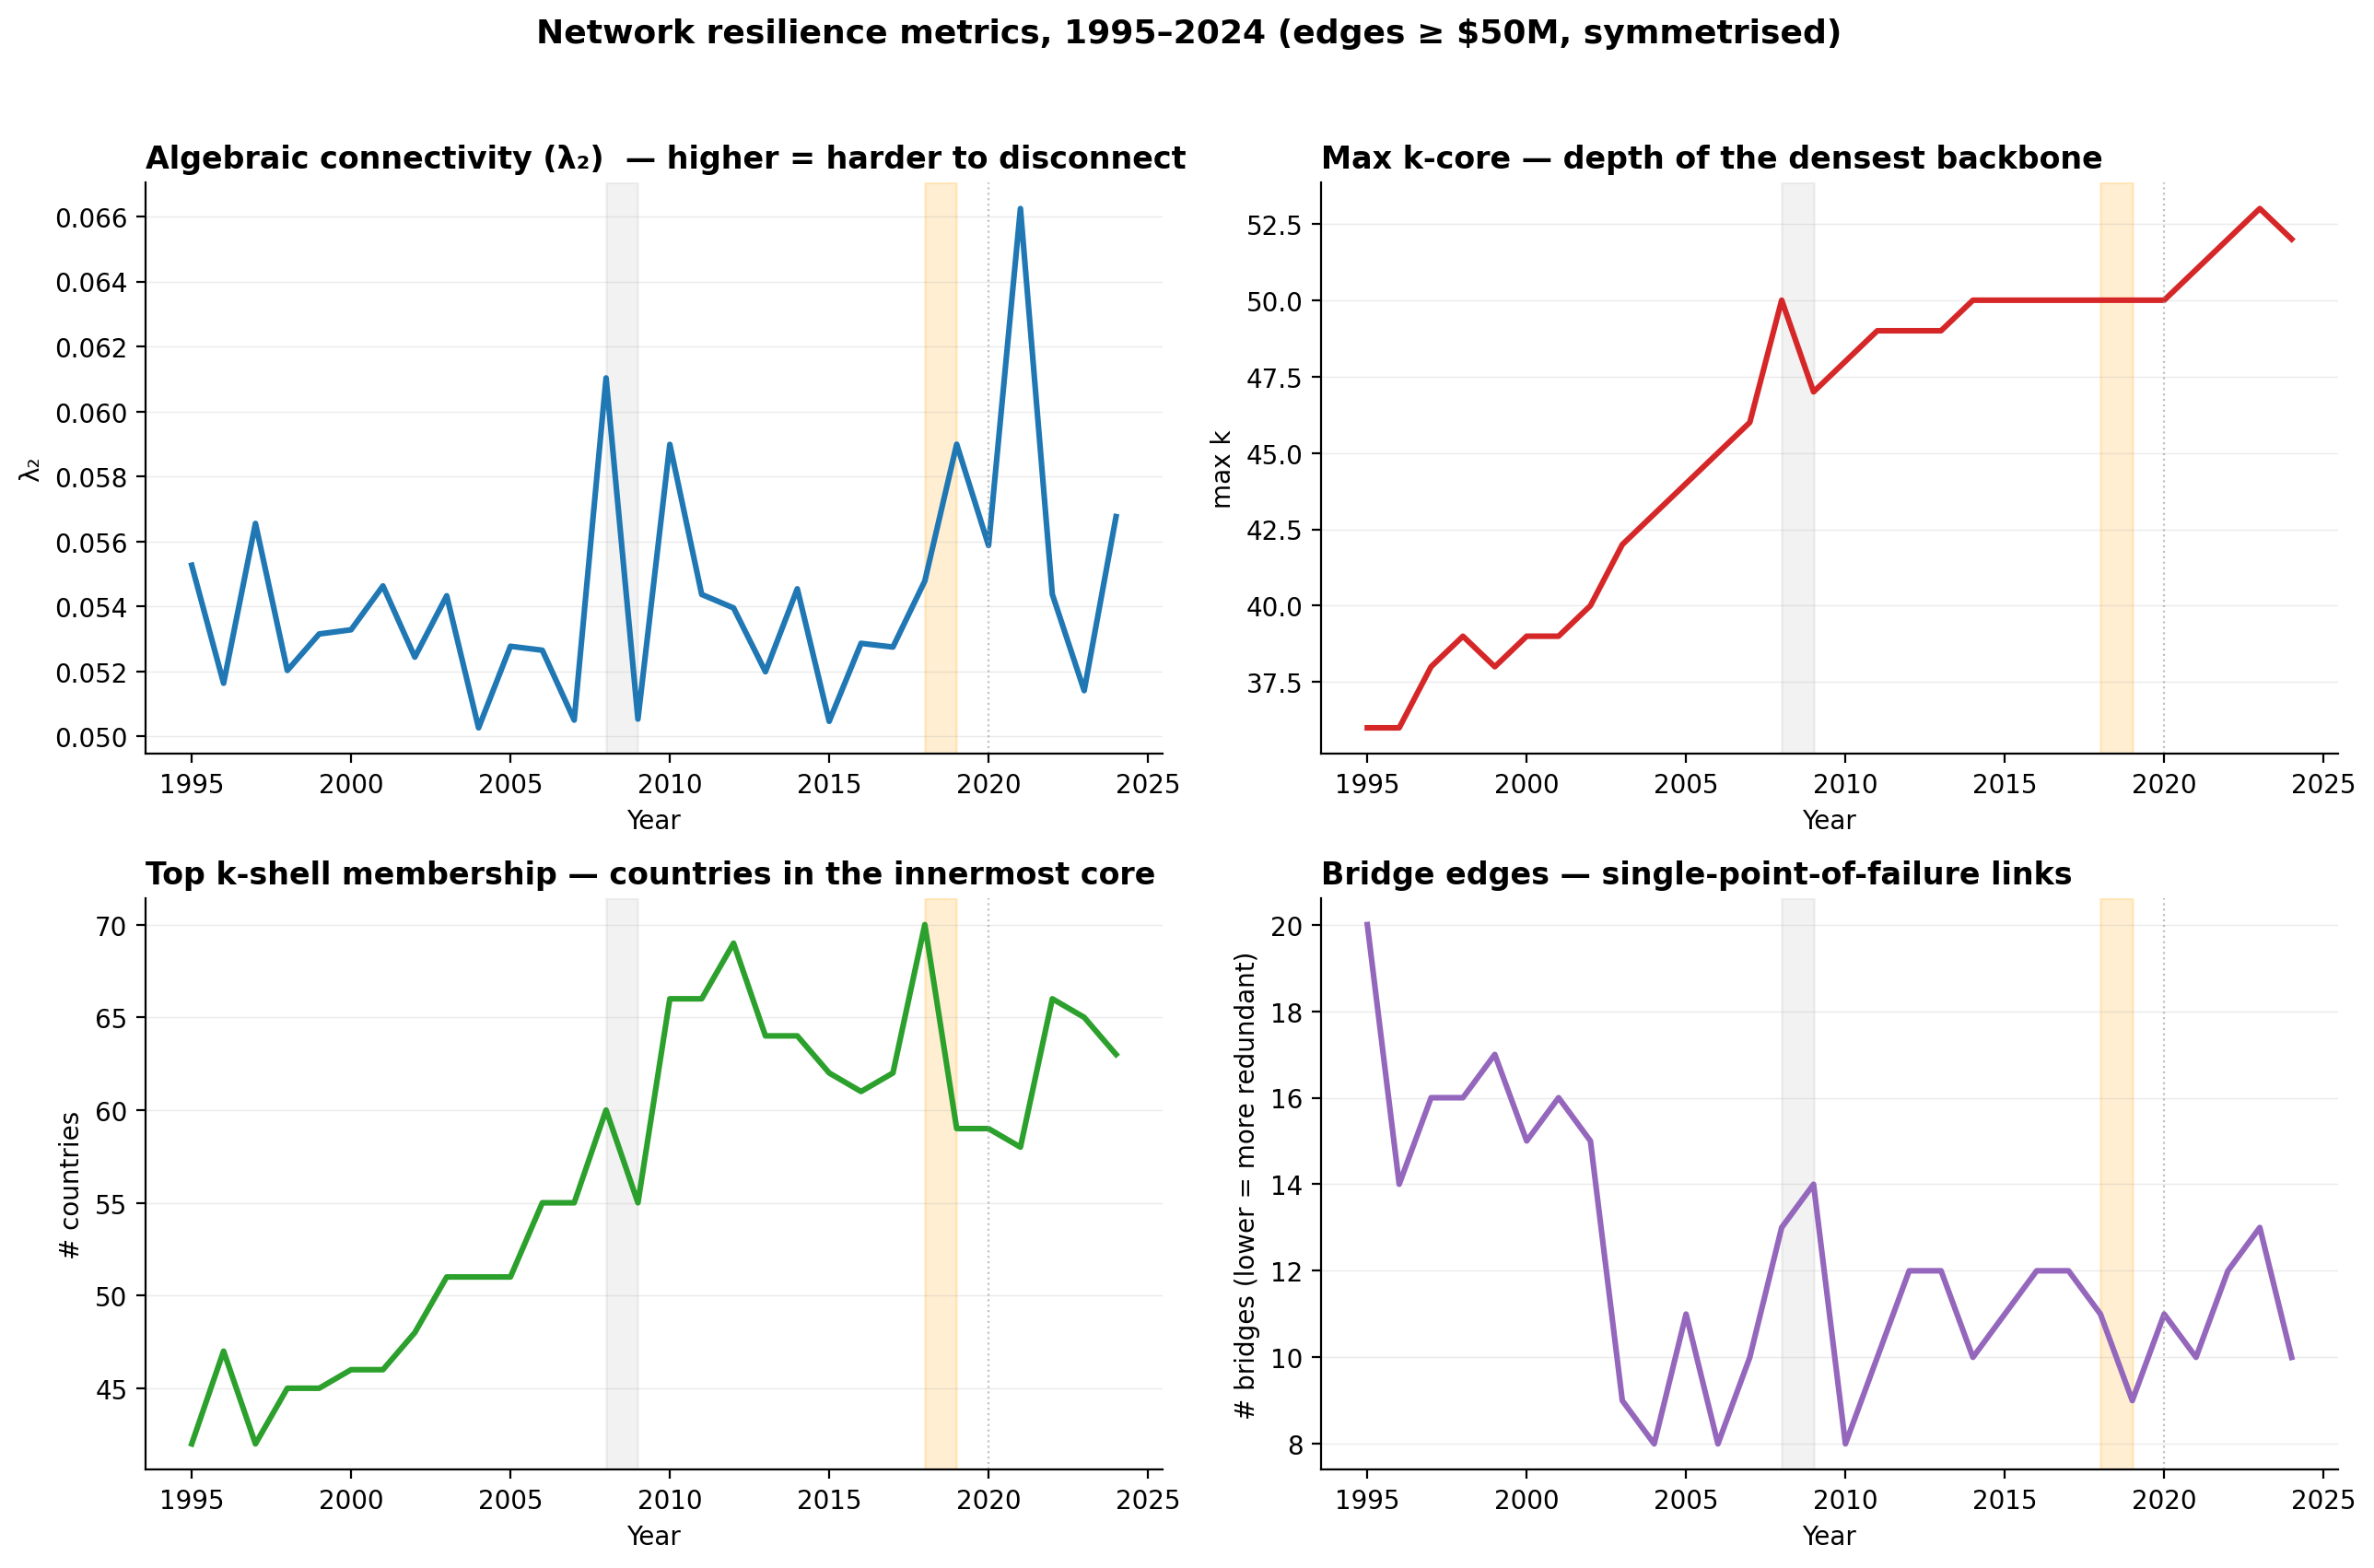
\includegraphics[width=\textwidth]{figures/fig13_resilience_metrics.png}
  \caption{Aggregate network resilience metrics, 1995--2024 (edges $\geq \$50$M, symmetrised).}
  \label{fig:res-agg}
\end{figure}

\begin{findbox}
\textbf{The aggregate network is remarkably robust and stayed that way
through the trade war.}

\begin{itemize}[leftmargin=*]
  \item $\lambda_2$ oscillates 0.05--0.07 with no trend; in fact \textbf{peaked
        in 2021} (post-COVID).
  \item Max k-core depth rose monotonically from 36 (1995) to 53 (2023):
        the backbone keeps deepening.
  \item Top k-shell membership peaked at 70 in 2018, then shrank to 63 by
        2024 — \textbf{the innermost core became slightly more exclusive}
        post-trade-war.
  \item Bridge edges stable at $\sim$10--15 (network has few single-point-of-failure links).
\end{itemize}
\end{findbox}

\begin{figure}[H]
  \centering
  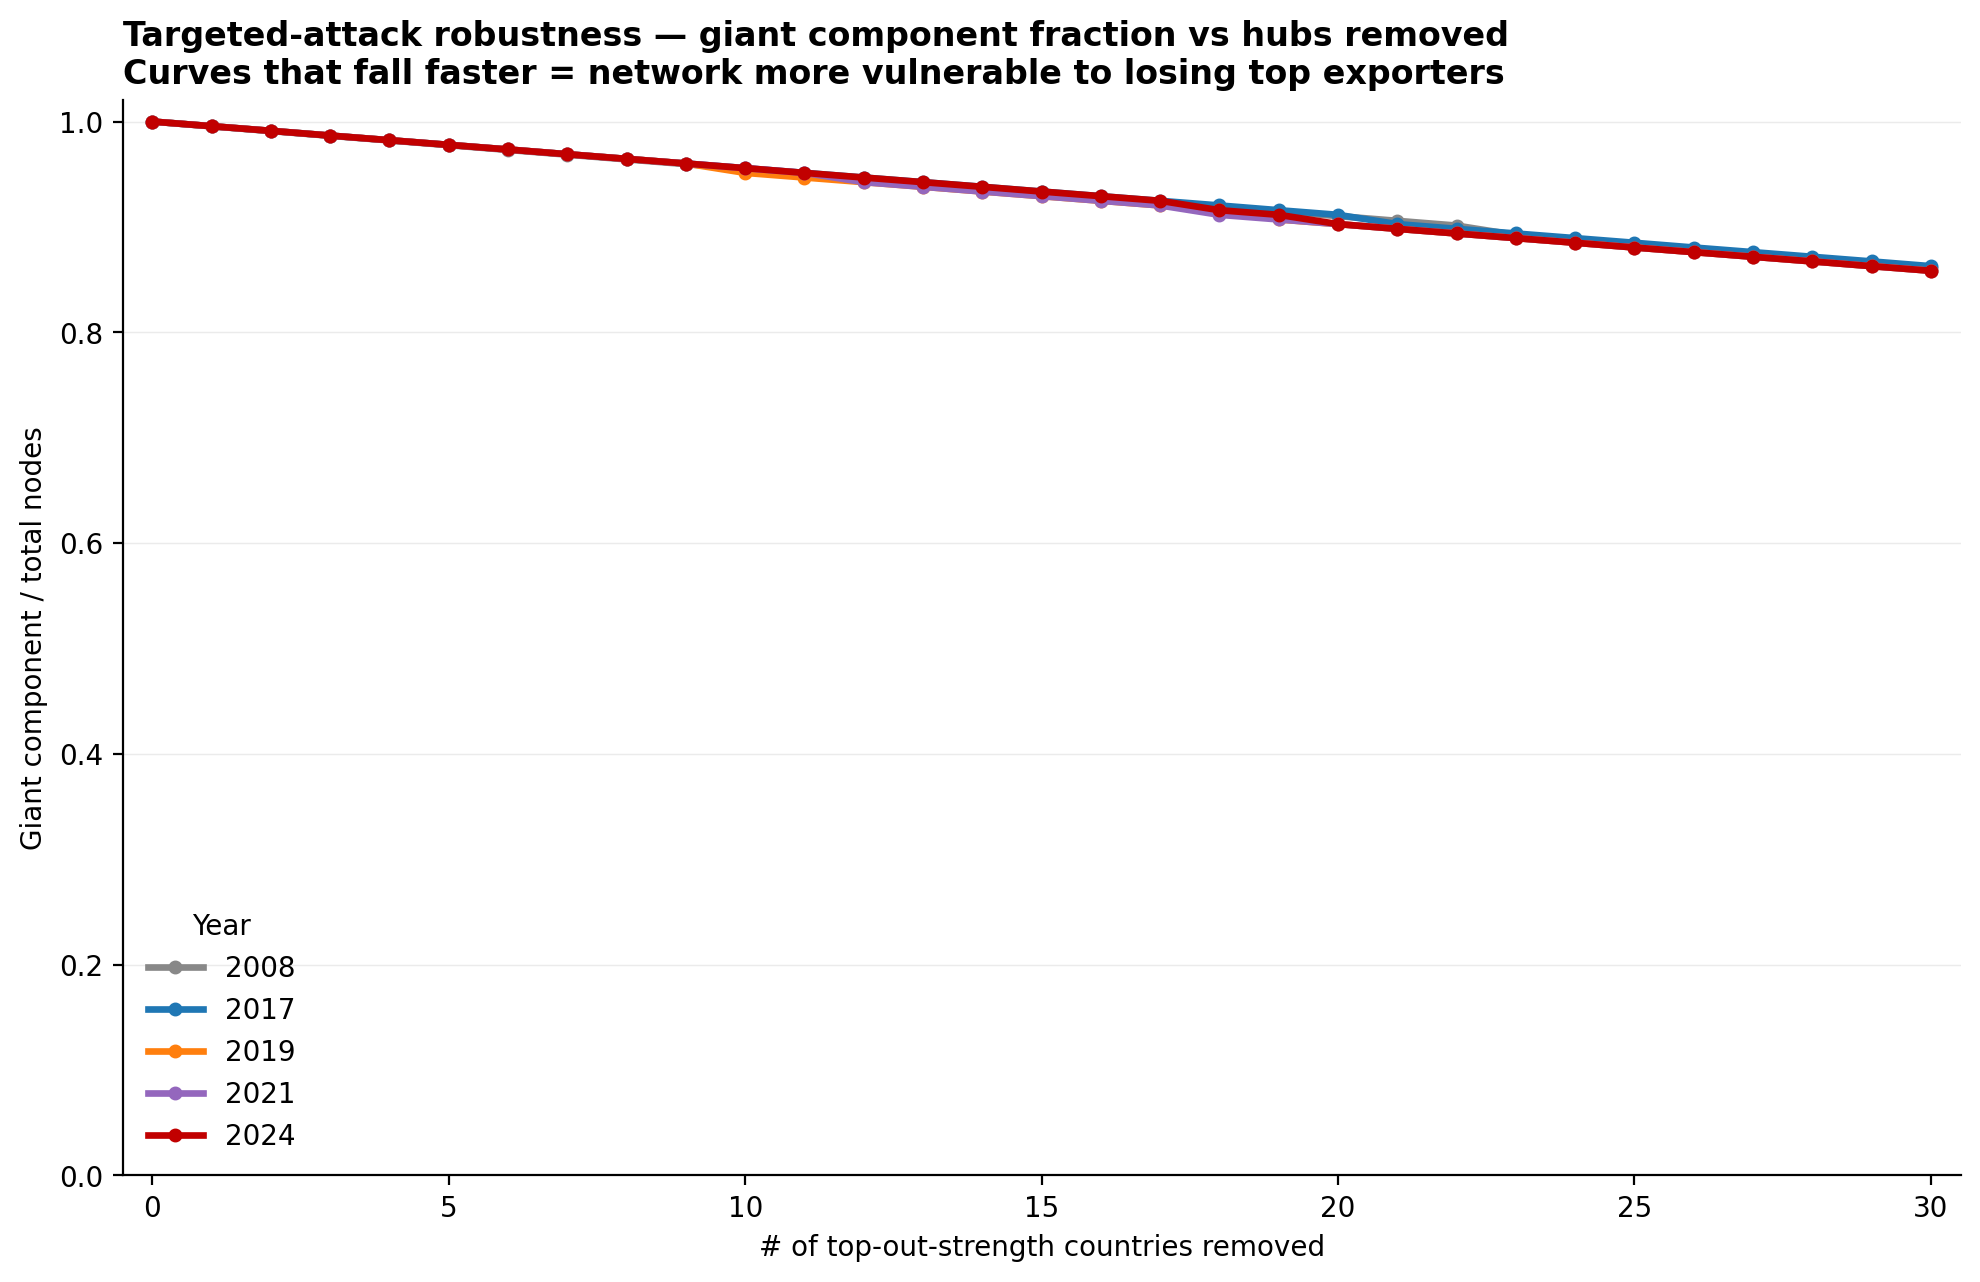
\includegraphics[width=0.9\textwidth]{figures/fig14_attack_robustness.png}
  \caption{Targeted-attack robustness: giant-component fraction as the top-$k$
  out-strength countries are removed. Curves are nearly indistinguishable
  across 2008, 2017, 2019, 2021, 2024 — \textit{the aggregate trade
  network's vulnerability to hub-removal did not change over this period.}}
\end{figure}

\subsection{Disaggregated resilience}

We re-ran the same pipeline on intermediate, capital, consumption and
semiconductor subnetworks (\texttt{resilience\_by\_subnetwork.py}) with
stage-appropriate edge thresholds.

\begin{figure}[H]
  \centering
  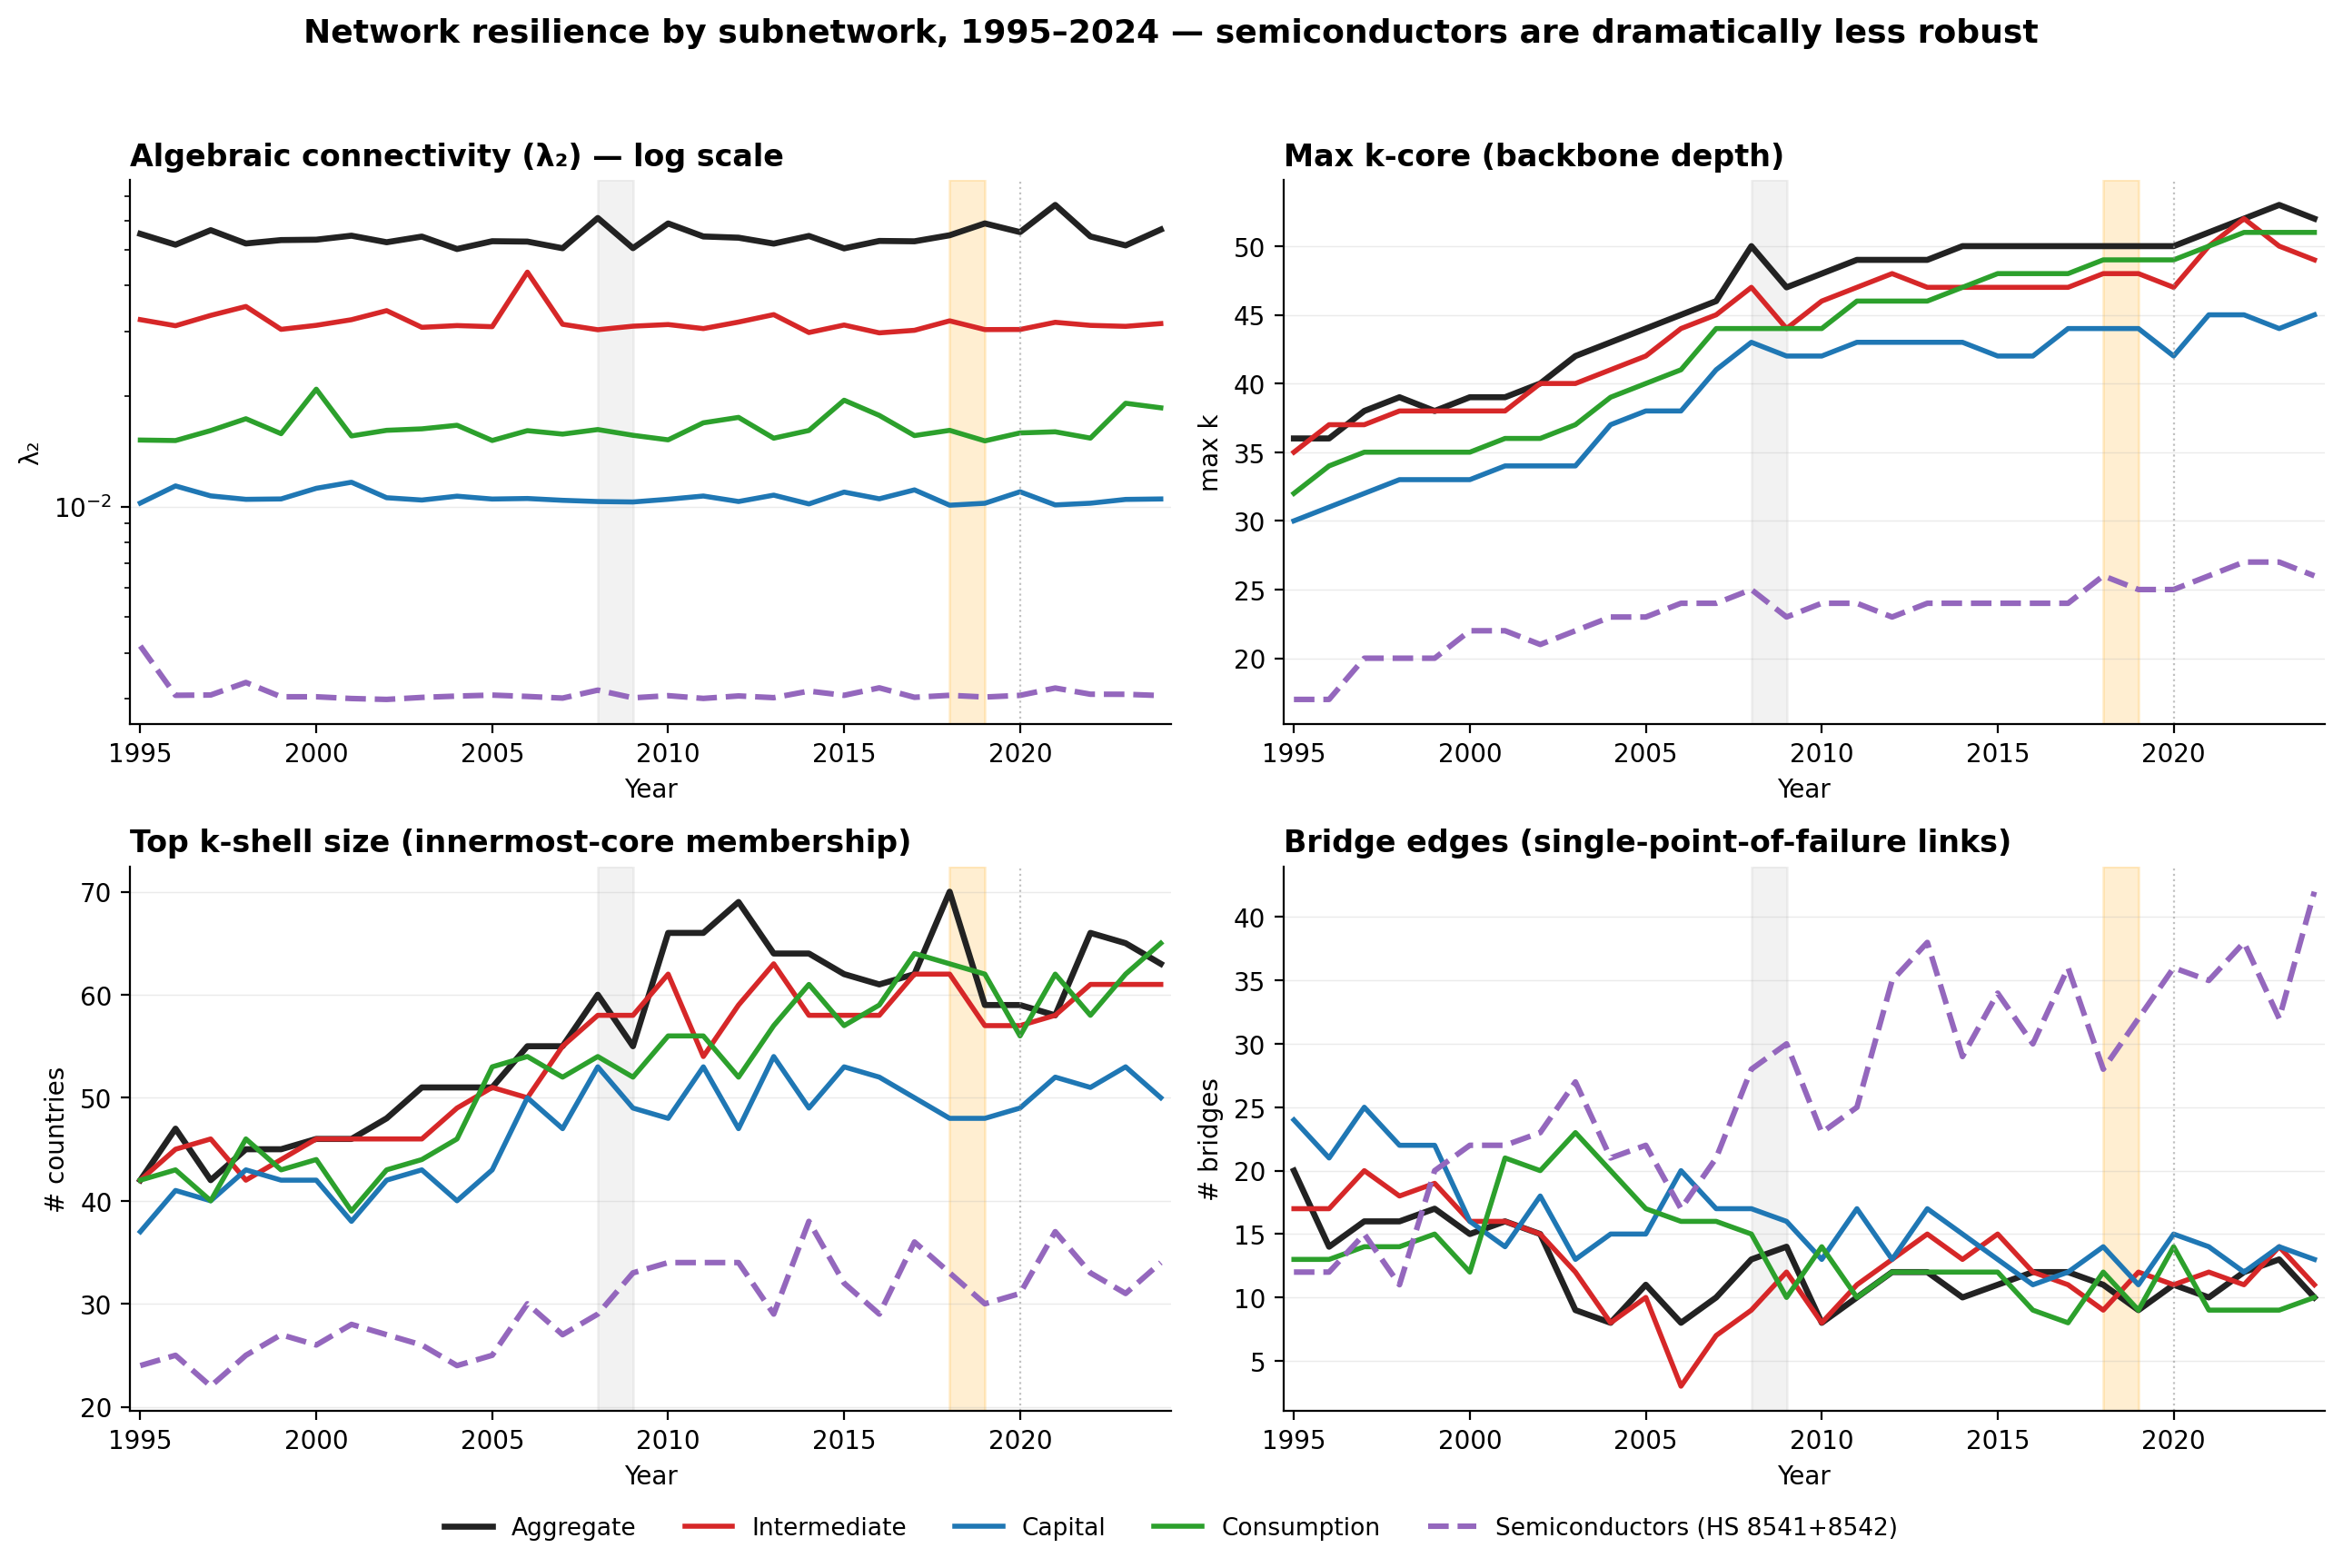
\includegraphics[width=\textwidth]{figures/fig17_resilience_compare_metrics.png}
  \caption{Resilience metrics by subnetwork, 1995--2024. The semiconductor
  network (dashed purple) is dramatically more fragile by every measure.}
  \label{fig:res-compare}
\end{figure}

\begin{figure}[H]
  \centering
  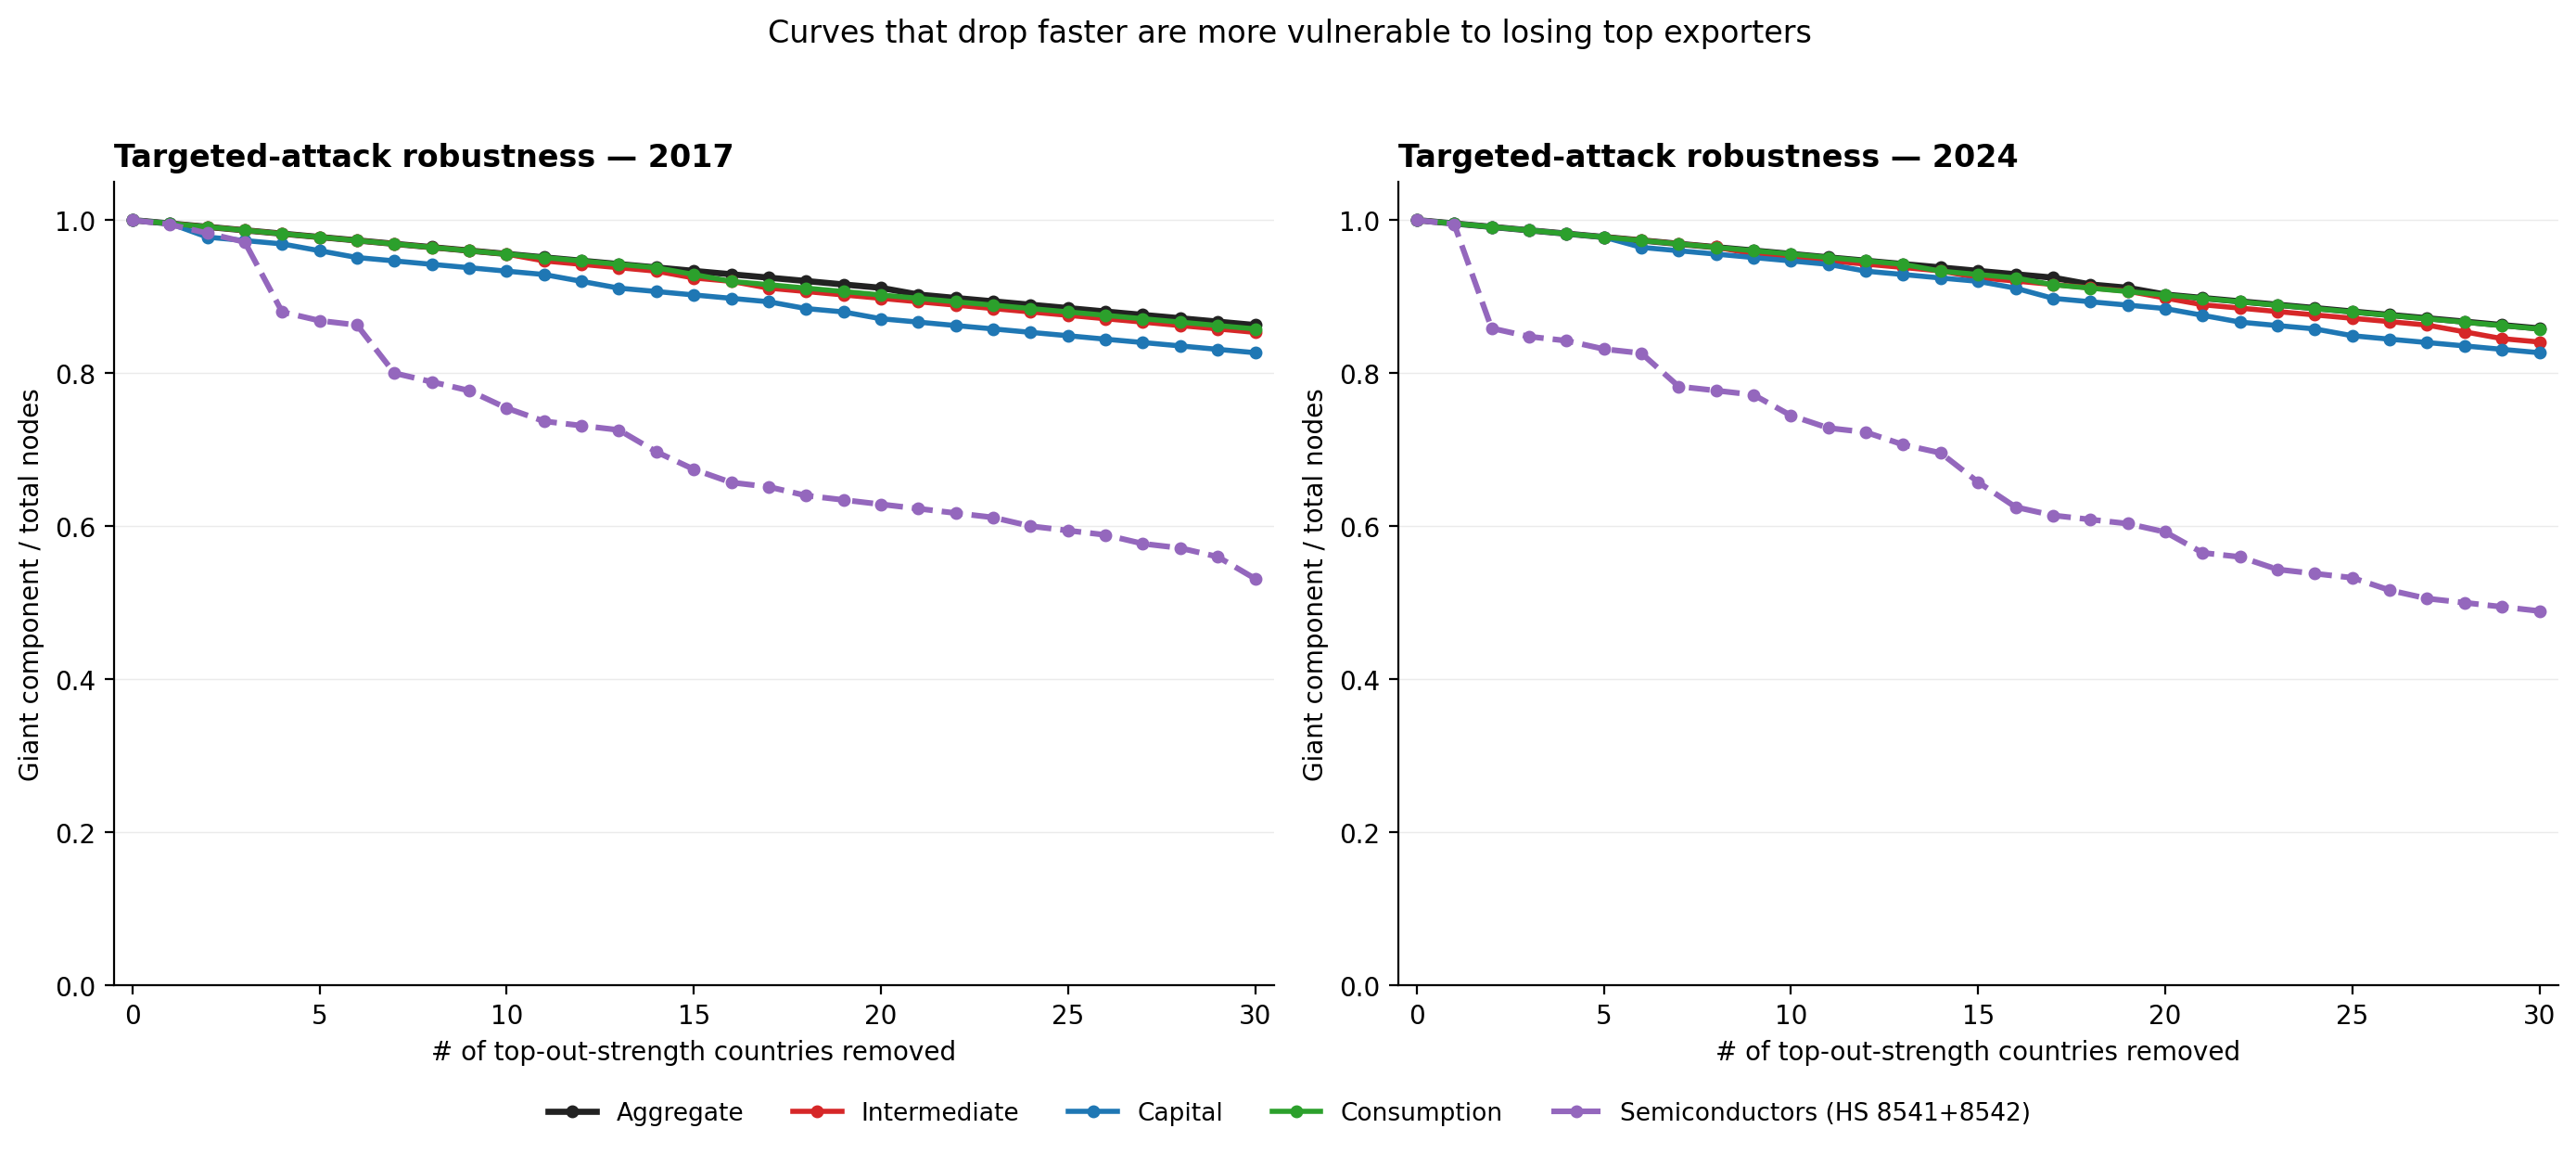
\includegraphics[width=\textwidth]{figures/fig18_resilience_compare_attack.png}
  \caption{Attack robustness curves by subnetwork in 2017 vs 2024.
  Semiconductor giant component collapses to $\sim$50\% after top-30
  removal in both years; aggregate stays above 85\%.}
  \label{fig:attack}
\end{figure}

\begin{findbox}
\textbf{The aggregate's apparent robustness hides stage-dependent fragility.}

A clear resilience hierarchy in 2024:
\begin{itemize}[leftmargin=*]
  \item Aggregate: $\lambda_2 = 0.057$, max k = 52, 10 bridges
  \item Intermediate: $\lambda_2 = 0.032$, max k = 49, 11 bridges
  \item Consumption: $\lambda_2 = 0.019$, max k = 51, 10 bridges
  \item \textbf{Capital}: $\lambda_2 = 0.011$, max k = 45, 13 bridges
  \item \textbf{Semiconductor}: $\lambda_2 = 0.003$, max k = 26, \textbf{42 bridges}
\end{itemize}

\textbf{Trade-war-era change (2017$\to$2024):}
Two stages worsened: capital marginally
($\lambda_2$ fell, bridges rose slightly), and semiconductors more
clearly (bridges 36$\to$42, top k-shell 36$\to$34). The other
three improved or stayed flat.
\end{findbox}

\subsection{The bridge-count caveat}

The 17\% rise in semiconductor bridges (36 $\to$ 42) is worth a careful
interpretation. Bridges are by definition periphery-to-core links — they
do not capture the dollar-weighted importance of edges. The increase is
\textit{partly mechanical}: the semiconductor network's node count grew
from 140 to 158 over this period, so more peripheral participants joined
with thin ties. A sharper supply-chain-fragility measure would be the
importer-side supplier-HHI (i.e., how dependent each importer is on its
single top supplier of each HS6).

\begin{limitbox}
\textbf{Cross-subnetwork comparisons are qualitative.} Different
edge-weight thresholds (\$50M aggregate down to \$3M for semiconductors)
mean the absolute values of $\lambda_2$ and density are not directly
comparable. \textit{Within-subnetwork temporal comparisons are reliable.}

\textbf{Semiconductor network has only 150 active nodes} (vs 215
aggregate); part of the lower $\lambda_2$ is mechanically due to smaller
network size, not just topology.

\textbf{Targeted attack uses out-strength.} PageRank or eigenvector
ordering would shift curves marginally; not tested.

\textbf{Static analysis} — no dynamic re-routing simulation. Real-world
disruption involves second-round substitution which is not modelled.
\end{limitbox}

% =====================================================================
\section{Summary of findings}

\begin{enumerate}[leftmargin=*]
  \item \textbf{Slowbalization of the aggregate trade network is real but
        predates the trade war.} Density plateaued circa 2010.
  \item \textbf{The trade war did not fragment the country-level trade
        network} (modularity slightly fell; communities stayed at 3--4).
        It did slightly contract the innermost core (70$\to$63 members
        2018$\to$2024).
  \item \textbf{China is the dominant network hub in 2024} (15.7\% of
        exports, betweenness 0.75). USA lost intermediary role.
  \item \textbf{Stage-specific specialisations are large and hidden by
        the aggregate}: China dominates \textit{capital} (22.6\%), not
        intermediates (12.5\%). Taiwan is 21\% of semiconductor exports.
  \item \textbf{Tariffs hit intermediates and consumption hardest} (78.9\%
        and 65.2\% of trade-value treated respectively); capital was
        largely spared (29.5\%). This is consistent with the policy
        intent of protecting US manufacturers' input access.
  \item \textbf{Global view of tariffed products shows China's share rose}
        — because of redirection to non-US markets. The US-side bilateral
        view is the right one for the diversion question.
  \item \textbf{US imports of tariffed products shifted clearly away from
        China} ($-\$24$B, $-6.1$ pp). Mexico (largest absolute gain),
        Korea, Vietnam, Taiwan (largest semi gain) absorbed the shift.
  \item \textbf{Vietnam's connector role is transshipment-flavoured}
        (China's share of Vietnam's intermediate imports of tariffed
        chapters rose from 30\% to 43\%).
  \item \textbf{Mexico's connector role is relocation-flavoured}
        (China share rose only +3.5 pp; intermediate-import base
        remains diversified).
  \item \textbf{Aggregate-network resilience did not degrade} through the
        trade war. The semiconductor subnetwork is structurally far more
        fragile than the aggregate, and got marginally more so post-2018.
        Capital goods showed a slight resilience decline.
\end{enumerate}

% =====================================================================
\section{Cross-cutting limitations}

\begin{enumerate}[leftmargin=*]
  \item \textbf{Gross trade, not value-added.} The single biggest
        limitation. All ``GVC-flavoured'' claims here are
        product-stage partitions of gross trade. The true value-added
        view requires input-output tables (TiVA / OECD ICIO / EXIOBASE).
  \item \textbf{HS92 vintage hides product detail for new categories.}
        Smartphones, lithium batteries, drones, advanced semiconductors
        are all somewhat bundled. PLAID-bridging at HS4 reduces this
        problem but does not eliminate it.
  \item \textbf{PLAID v0.1 has no formal methodology paper available
        to us}; we take its classifications at face value.
  \item \textbf{Tariff data covers only 4{,}726 HS6 codes} (FGKK 2023
        universe). HS6 codes not in FGKK are treated as untreated by
        default.
  \item \textbf{Static network analysis.} No dynamic shock-propagation
        simulation, no second-round substitution, no demand-side elasticities.
  \item \textbf{Bridge count is a topological measure}; it does not weight
        by trade value. Many semiconductor bridges are between core
        countries and small peripheral participants and have minor
        substantive importance.
  \item \textbf{No causal identification.} Everything in this document is
        descriptive. Causal trade-war effects would require either
        a difference-in-differences design (e.g., Fajgelbaum et al. 2020)
        or a structural estimation. This work establishes the
        descriptive ground; causal work could build on top.
\end{enumerate}

% =====================================================================
\section{Data warnings and items to double-check}
\label{sec:warnings}

This section lists open questions about the underlying data that should be
verified before any finding above is cited or built upon. They are flagged
explicitly so that no result silently rests on an unverified assumption.
Each warning is independent and is grouped by topic.

\subsection*{W.1 The 2024 anomaly}

\begin{warnbox}
Several headline metrics show an unusual move in 2024:
\begin{itemize}[leftmargin=*]
  \item Aggregate trade-network edge count fell by 4.6\% versus 2023
        (the largest year-on-year decline outside the 2008--09 GFC and
        the 2020 COVID shock).
  \item Year-on-year edge-set Jaccard dropped to 0.844 — the lowest
        value since 1996.
  \item The semiconductor subnetwork shrank similarly ($-5.9$\% edges).
\end{itemize}
\textbf{Possible causes}: (a) a real structural break — early Trump-II
positioning, semiconductor export controls, anticipatory shifts.
(b) An artefact of incomplete 2024 reporting in BACI V202601 — CEPII
typically releases revisions of the most recent year a year or two later
as more national customs data is reconciled.
\textbf{Action required}: check CEPII's release notes for BACI V202601
to confirm 2024 coverage is comparable to earlier years; rerun the
key 2024 metrics on a future BACI vintage when available.
\textbf{Affects}: any claim about ``the 2024 contraction.''
\end{warnbox}

\subsection*{W.2 HS4 aggregation of PLAID and within-chapter heterogeneity}

\begin{warnbox}
PLAID v0.1 is in HS2022; BACI HS92 V202601 is in HS92. Direct HS6 merge
gives only 75\% trade-value coverage. We bridge this by aggregating
PLAID to HS4 chapter level, which raises coverage to 99\%.
\textbf{Cost}: each HS6 inherits its HS4 chapter's averaged BEC / Rauch
share, which loses precision for chapters with heterogeneous internal
PLAID classifications.
\textbf{Quantitative check}: $1{,}097$ of $1{,}229$ HS4 chapters
($\approx$89\%) have a single dominant BEC class with at least 80\%
modal-class share. The remaining $\approx$11\% of HS4 chapters
contribute composition noise to the BEC-stage aggregates.
\textbf{Affects}: BEC-stratified network metrics (Section 5),
specialisation heatmap (Section 7), friend-shoring HS4 results.
\textbf{Mitigation}: the friend-shoring HS6 analysis (Section 8) uses
PLAID at HS6 directly and explicitly handles the 25\% missing share.
\end{warnbox}

\subsection*{W.3 FGKK tariff universe is partial}

\begin{warnbox}
The FGKK \texttt{z\_usch\_w} file covers 4{,}726 HS6 codes
(of $\sim$5{,}022 in BACI HS92). HS6 codes not in FGKK default to
``untreated'' in our tariff partitions.
\textbf{Affects}: the binary tariff-stratified subnetworks
(Section~6). Trade in HS6 codes outside the FGKK universe is counted as
``untreated'' even if the products were in fact subject to Section 301
tariffs not captured by FGKK's HS reconciliation.
\textbf{Action}: cross-check against the USITC HTS tariff schedule for
material discrepancies; estimate the magnitude of misclassified trade.
\end{warnbox}

\subsection*{W.4 Tariff variable interpretation
($z_{usch,w}$ versus $dz_{usch,w}$)}

\begin{warnbox}
$z_{usch,w}(t=1)$ is the post-period weighted tariff level and includes
any pre-existing MFN baseline. $dz_{usch,w}$ is the change versus
$t=-1$ (the trade-war-induced increment). We verified that the
two definitions of ``treated'' yield essentially the same set
($4{,}428$ vs $4{,}411$ HS6 codes — only 17 difference).
\textbf{Action}: in any regression-style analysis, use
$dz_{usch,w}$ as the change variable rather than the level
$z_{usch,w}$, to capture only the trade-war-induced variation.
\end{warnbox}

\subsection*{W.5 HS 854140 mixes photovoltaic cells with LEDs}

\begin{warnbox}
The narrow semiconductor filter (HS 8541+8542) includes HS 854140,
which lumps photovoltaic cells / solar modules with light-emitting
diodes (and photo-sensitive semiconductor devices).
\textbf{Impact}: China dominates solar; some Chinese ``semiconductor''
share in our HS 8541+8542 filter is in fact solar.
\textbf{Mitigation}: as a robustness check, rerun the semiconductor
analysis on HS 8542 only (integrated circuits) to isolate the
``real chips'' story.
\end{warnbox}

\subsection*{W.6 PLAID v0.1 has no methodology paper available}

\begin{warnbox}
PLAID is marked ``v0.1'' and we use it without a peer-reviewed
methodology document. We accept its HS6-level classifications at face
value.
\textbf{Action}: locate or request the methodology / construction notes
from the PLAID authors before citing PLAID-derived classifications in a
final thesis chapter.
\end{warnbox}

\subsection*{W.7 PLAID's microchip indicator is too broad}

\begin{warnbox}
PLAID's binary \texttt{microchip\_content} flag classifies as ``contains
microchips'' a wide range of products including washing machines,
dishwashers, bulldozers and marine diesel engines (because these contain
embedded electronics). This is technically correct but useless for
analyses focused on semiconductors or strategic-tech goods.
\textbf{Mitigation}: we replaced PLAID's microchip indicator with a
direct HS 8541+8542 filter (Section~B.3). Any earlier or auxiliary
analyses using \texttt{long\_run\_metrics\_microchip.py} should be read
as ``trade in goods containing embedded electronics,'' not
``semiconductors.''
\end{warnbox}

\subsection*{W.8 Resilience thresholds differ across subnetworks}

\begin{warnbox}
The resilience pipeline drops edges below a network-specific dollar
threshold to obtain a meaningful sparse graph for k-core / $\lambda_2$
computation. Thresholds: \$50M (aggregate), \$30M (intermediate),
\$15M (consumption), \$10M (capital), \$3M (semiconductor).
\textbf{Implication}: absolute values of $\lambda_2$, density and
bridge counts are \emph{not directly comparable} across subnetworks.
\textbf{Within-subnetwork temporal comparisons are reliable;
cross-subnetwork comparisons are qualitative only.}
\end{warnbox}

\subsection*{W.9 Bridge count is a topological measure, not a
supply-chain-fragility measure}

\begin{warnbox}
A ``bridge'' is an edge whose removal disconnects the network. In trade
networks, almost all bridges are periphery-to-core ties: a small
participating country's only above-threshold trade link.
The reported 17\% increase in semiconductor bridges (36$\to$42, 2017
to 2024) is partly mechanical — the semiconductor network's node count
grew from 140 to 158 over that period, so more peripheral participants
joined with thin ties.
\textbf{Bridge count is not a direct supply-chain-fragility statistic.}
A sharper measure is the per-importer supplier-HHI (concentration of
each importer's supply mix per HS6).
\end{warnbox}

\subsection*{W.10 Country code S19 = Taiwan in BACI}

\begin{warnbox}
The BACI nomenclature uses ISO3 code \texttt{S19} (``Other Asia, nes'')
for Taiwan rather than \texttt{TWN}, consistent with UN Comtrade
convention. There is no separate \texttt{TWN} record.
\textbf{Action}: any downstream analysis that filters by country code
must use \texttt{S19} for Taiwan. Confusing this would dramatically
under-state Taiwan's role in the semiconductor network (S19 holds 21.4\%
of global semiconductor exports in 2024).
\end{warnbox}

\subsection*{W.11 Tariff time coverage stops at Dec 2019; BACI extends to 2024}

\begin{warnbox}
The FGKK monthly retaliatory tariff file (\texttt{z\_chus}) covers
2018-04 through 2019-12 only. The collapsed three-period file
(\texttt{z\_usch\_w}) compresses pre / transition / post into three
discrete moments. There is no high-frequency tariff variation past the
Phase 1 deal (January 2020).
\textbf{Implication}: post-2020 BACI data reflects ``treatment frozen''
status. Any post-COVID restructuring is intermingled with COVID,
inflation, Ukraine and Red Sea shocks. The trade-war ``post period''
is not cleanly identified after 2019.
\end{warnbox}

\subsection*{W.12 TiVA FDVA cache only covers 2019--2022 at activity level}

\begin{warnbox}
The local TiVA Foreign Direct Value Added cache
(\texttt{tiva\_fdva\_cache/}) has activity-level data only for
2019--2022. There is no pre-trade-war (2017) FDVA snapshot in the
current pull. Any future ``BACI vs TiVA value-added'' cross-check
needs to extend \texttt{fdva\_network.py} to additional years (the
OECD SDMX API supports 1995 onwards at $\_T \times \_T$ level).
\textbf{Action}: extend the cache before doing the cross-validation
step in Phase E.
\end{warnbox}

\subsection*{W.13 The displacement vs.\ diversion confound in
``treated trade'' global network metrics}

\begin{warnbox}
Section 6 (tariff-stratified subnetworks) operates on \emph{global}
bilateral trade in tariff-treated HS6 codes. This pools two distinct
mechanisms:
\begin{enumerate}[leftmargin=*]
  \item Diversion: US imports of treated products from China fall,
        partially replaced by imports from other sources.
  \item Displacement: Chinese exports of treated products are
        redirected from the US toward non-US destinations.
\end{enumerate}
These two cannot be separated at the global-network level. The
counter-intuitive finding that ``China's global share rose in
high-tariff products'' is consistent with strong displacement plus
moderate diversion — but the network-level view alone cannot quantify
either component.
\textbf{Mitigation}: the US-as-importer friend-shoring analysis (Section 8)
isolates the diversion mechanism.
\textbf{Future work}: a symmetric analysis with China-as-importer
(using $z_{chus}$) would isolate the displacement story.
\end{warnbox}

\subsection*{W.14 No 2025 data; Trump-II tariffs are out of sample}

\begin{warnbox}
BACI V202601 ends in 2024. The 2025 Trump-administration tariff wave
(announced April 2025, ramping through summer 2025) is not yet
observable in the data. Any statements about resilience going into the
``second wave'' are forward-looking and speculative.
\end{warnbox}

\subsection*{W.15 Static analysis throughout}

\begin{warnbox}
All findings are descriptive cross-sections or time-series of the
trade-flow network. We do not simulate dynamic shock propagation, second-round
supplier substitution, or demand-side elasticities.
A node-removal in the attack curves is a hypothetical static test, not
a forecast of actual disruption response.
\textbf{Affects}: any claim about ``what would happen if China
stopped exporting product X.''
\end{warnbox}

\subsection*{W.16 No causal identification}

\begin{warnbox}
This document is entirely descriptive. Causal trade-war effects would
require either a difference-in-differences design
(e.g., Fajgelbaum, Goldberg, Kennedy \& Khandelwal 2020) or a
structural estimation. The present work establishes the descriptive
ground; causal work would build on top.
\end{warnbox}

\subsection*{Quick-action priority}

If only one or two warnings can be addressed before write-up, prioritise:
(1) verifying BACI 2024 coverage with CEPII (W.1) — without this, the
2024 contraction finding is contingent;
(2) confirming the FGKK tariff coverage against the USITC HTS schedule
(W.3) — without this, the ``treated'' set may be partial;
(3) extending the TiVA FDVA cache to 2017 (W.12) — without this, no
value-added cross-validation is possible.

% =====================================================================
\section{Pipeline reference}

For reproducibility, the code repository contains the following scripts
(all in the project root, run with the Anaconda Python 3 distribution):

\begin{itemize}[leftmargin=*,itemsep=2pt]
  \item \texttt{build\_baci\_artifacts.py} — builds
        \texttt{baci\_combined.parquet} and \texttt{baci\_edges\_country.parquet}
        from per-year BACI parquets (streaming, 16~GB-RAM-safe).
  \item \texttt{build\_plaid\_edges.py} — merges PLAID at HS4 and
        emits BEC / Rauch / microchip stratified edge lists.
  \item \texttt{build\_tariff\_master.py} — pivots FGKK tariff data and
        merges with PLAID to produce \texttt{hs4\_master.csv}.
  \item \texttt{build\_tariff\_edges.py} — partitions BACI by tariff
        treatment status.
  \item \texttt{build\_semi\_edges.py} — narrow HS 8541+8542 filter.
  \item \texttt{long\_run\_network\_metrics.py} (with reusable
        \texttt{run\_long\_run}) — annual network metrics pipeline.
  \item \texttt{long\_run\_metrics\_by\_bec.py} /
        \texttt{long\_run\_metrics\_semi.py} /
        \texttt{long\_run\_metrics\_tariff.py} — stratified runs.
  \item \texttt{resilience\_aggregate.py} (with reusable
        \texttt{run\_resilience}) — k-core, $\lambda_2$, attack curves,
        backbone extraction.
  \item \texttt{resilience\_by\_subnetwork.py} — same on stratified subnetworks.
  \item \texttt{viz\_bec\_comparison.py} — figures 1--5.
  \item \texttt{viz\_added\_value.py} — figures 6--8.
  \item \texttt{viz\_tariff\_strata.py} — figures 9--10.
  \item \texttt{viz\_friendshoring\_hs6.py} — figures 11--12.
  \item \texttt{viz\_resilience.py} — figures 13--16.
  \item \texttt{viz\_resilience\_compare.py} — figures 17--18.
  \item \texttt{tables\_friendshoring.py} — friend-shoring tables (CSV).
\end{itemize}

% =====================================================================
\section{Suggested next steps}

\begin{enumerate}[leftmargin=*]
  \item \textbf{Importer-side supplier-HHI} per HS6 — sharper
        supply-chain-fragility metric than bridge count.
  \item \textbf{Hub-removal cascade simulation}: actually remove China
        from each 2024 subnetwork, allocate disrupted trade by reweighting,
        measure stranded volume by country. Direct ``what-if'' policy answer.
  \item \textbf{Mirror friend-shoring analysis using Chinese retaliatory
        tariffs} (\texttt{z\_chus}): did Chinese imports of US-targeted
        products shift away from USA toward Brazil/Australia/EU?
  \item \textbf{TiVA cross-check} on the key bilateral pairs
        (CHN--USA, CHN--VNM, VNM--USA, CHN--MEX, MEX--USA) — the only
        way to convert circumstantial transshipment vs relocation
        signals into value-added evidence.
  \item \textbf{NLP-derived continuous upstreamness} at HS6 — a
        thesis-grade methodological contribution that current literature
        lacks.
\end{enumerate}

% =====================================================================
\appendix
\section*{Appendix: Glossary of network-theoretic methods}
\addcontentsline{toc}{section}{Appendix: Glossary of network-theoretic methods}

This appendix defines each network-theoretic concept used in the analysis.
Each entry has three parts: (1) a plain-language description, (2) the
formal definition / formula, and (3) an interpretation note describing what
high or low values mean and where in the analysis the measure is used.

\subsection*{A.1\quad Network basics}

\textbf{Trade network as a directed weighted graph.}
We represent the world trade system as a graph $G = (V, E, w)$ where
$V$ is the set of $n \approx 230$ countries (nodes), $E \subseteq V \times V$
is the set of ordered country pairs with non-zero bilateral trade in a given
year (directed edges), and $w: E \to \mathbb{R}_+$ assigns each edge its
bilateral trade value in USD.
For some metrics (k-core, Laplacian-based measures, community detection)
we work on a \emph{symmetrised undirected} graph $\tilde{G}$ where the
edge between $u$ and $v$ has weight
$\tilde{w}(u,v) = w(u,v) + w(v,u)$.

\paragraph{Density.}
The fraction of all possible edges that actually exist.
\[
\rho_{\text{directed}} = \frac{|E|}{n(n-1)},
\qquad
\rho_{\text{undirected}} = \frac{2|E|}{n(n-1)}.
\]
\emph{Interpretation}: $\rho = 0$ (no edges), $\rho = 1$ (complete graph).
A higher density means countries are, on average, more interconnected in
bilateral trade. In our analysis density indicates how globalised the trade
network is.

\paragraph{Degree and strength.}
The \emph{out-degree} of node $v$ is the number of countries it exports
to: $d_v^{\text{out}} = |\{u : (v,u) \in E\}|$. The \emph{in-degree} is
the number it imports from. The \emph{out-strength} is the
weight-summed version:
\[
s_v^{\text{out}} = \sum_{u : (v,u) \in E} w(v,u),
\qquad
s_v^{\text{in}} = \sum_{u : (u,v) \in E} w(u,v).
\]
\emph{Interpretation}: out-strength is total exports; in-strength is total
imports. In our country-share figures, the share of a country is its
out-strength divided by the global out-strength sum.

\subsection*{A.2\quad Centrality measures}

\paragraph{PageRank (Brin \& Page 1998).}
Probability that a ``random walker'' who follows edges proportional to
their weight (with a small probability of teleporting to a random node)
ends up at a given node in the stationary distribution. For damping
parameter $\alpha \in (0,1)$ (we use $\alpha = 0.85$):
\[
r(v) = \alpha \sum_{u : (u,v) \in E} \frac{w(u,v)}{s_u^{\text{out}}}\, r(u)
\;+\; (1-\alpha)\frac{1}{n}.
\]
\emph{Interpretation}: a country's PageRank is high if it is the
destination of many high-weight flows from other countries that
themselves have high PageRank. Higher = more centrally embedded.

\paragraph{Eigenvector centrality.}
A node's centrality is proportional to the centrality of its neighbours.
Formally, the centrality vector $\mathbf{e}$ is the eigenvector of the
weighted adjacency matrix $A$ associated with its largest eigenvalue
$\lambda_{\max}$:
\[
\lambda_{\max}\, e(v) = \sum_{u} A_{uv}\, e(u).
\]
\emph{Interpretation}: similar to PageRank but without teleportation;
emphasises being connected to other already-important countries.

\paragraph{Betweenness centrality (Freeman 1977).}
Fraction of shortest paths between other node pairs that pass through
node $v$. For weighted networks we use the reciprocal of weight as
``distance'' so heavy edges count as short paths:
\[
b(v) = \sum_{\substack{s \neq v \neq t}} \frac{\sigma_{st}(v)}{\sigma_{st}},
\]
where $\sigma_{st}$ is the number of shortest paths from $s$ to $t$, and
$\sigma_{st}(v)$ the number that pass through $v$.
\emph{Interpretation}: high betweenness = a country sits on many trade
routes between others, i.e.\ plays a hub/intermediary role. In our
analysis, USA's betweenness fell from 0.66 (1995) to 0.42 (2024); China's
rose from 0.03 to 0.75.

\subsection*{A.3\quad Community structure}

\paragraph{Modularity (Newman \& Girvan 2004).}
For a partition $\mathcal{C} = \{C_1, \dots, C_k\}$ of $V$ into communities,
modularity measures how much the within-community link density exceeds
what would be expected by chance under a degree-preserving null model:
\[
Q = \frac{1}{2m} \sum_{u,v}
\left[ A_{uv} - \frac{d_u d_v}{2m} \right]\delta(c_u, c_v),
\]
where $A_{uv}$ is the (weighted) adjacency, $d_u = \sum_v A_{uv}$, $m =
\tfrac{1}{2}\sum_{u,v} A_{uv}$ is the total weight, and $\delta(c_u, c_v)
= 1$ if $u$ and $v$ are in the same community (else $0$).
\emph{Interpretation}: $Q \approx 0$: no community structure. $Q > 0.3$
typically indicates meaningful community structure. Higher = more bloc-y.
In our analysis the aggregate trade-network modularity oscillates around
0.26 since 2018, with no sharp break, contradicting the
``trade-war-fragmented-the-network'' narrative.

\paragraph{Louvain algorithm (Blondel et al.\ 2008).}
A fast greedy heuristic that finds a partition $\mathcal{C}$ with high
$Q$. Iterates two phases until $Q$ no longer improves:
(1) each node tentatively moves to a neighbour's community if the move
increases $Q$;
(2) communities are aggregated into super-nodes and the process repeats.
We use the networkx implementation with a fixed random seed for
reproducibility.

\subsection*{A.4\quad Concentration and edge-set similarity}

\paragraph{Herfindahl--Hirschman Index (HHI).}
Standard concentration measure used in industrial economics.
\[
\mathrm{HHI} = \sum_{v \in V} s_v^2,
\qquad
s_v = \frac{s_v^{\text{out}}}{\sum_{u} s_u^{\text{out}}}.
\]
\emph{Interpretation}: $\mathrm{HHI} \in [1/n, 1]$.
$\mathrm{HHI} = 1/n$ corresponds to perfectly equal market shares;
$\mathrm{HHI} = 1$ to a monopoly.
US DOJ thresholds for market concentration: $<0.15$ unconcentrated, $0.15$--$0.25$
moderately concentrated, $>0.25$ highly concentrated.
We use it both at network level (concentration of out-strength shares
across countries) and at importer-product level (supplier concentration).

\paragraph{Jaccard similarity.}
For two sets $A$ and $B$:
\[
J(A, B) = \frac{|A \cap B|}{|A \cup B|}.
\]
\emph{Interpretation}: $1$ = identical, $0$ = disjoint. We use it
year-over-year on the edge set: a high Jaccard means the network's link
structure (which pairs trade) is stable from one year to the next; a
falling Jaccard signals real bilateral restructuring.

\subsection*{A.5\quad Robustness and resilience}

\paragraph{Largest weakly connected component (WCC).}
A directed graph is \emph{weakly connected} if its underlying undirected
graph is connected. The \emph{largest WCC} is the largest such connected
piece. Its size relative to $|V|$ is a basic measure of cohesion:
$|V_{\text{WCC}}|/|V| = 1$ means the graph is fully connected.

\paragraph{Bridge edge.}
An edge $e \in E$ is a \emph{bridge} if its removal increases the number
of connected components of the underlying undirected graph.
\emph{Interpretation}: bridges are single-point-of-failure links.
In trade networks they are almost always at the periphery (a small
country whose only above-threshold trade tie is to a single hub).
A higher bridge count means more peripheral fragility, not necessarily
deeper supply-chain vulnerability.

\paragraph{k-core decomposition (Seidman 1983).}
Iteratively remove all nodes of degree $<k$. The remaining maximal
subgraph in which every node has degree $\geq k$ is the \emph{k-core}.
The \emph{core number} of node $v$ is the largest $k$ such that $v$ still
belongs to the $k$-core:
\[
c(v) = \max\{k : v \in \text{k-core}(\tilde{G})\}.
\]
The \emph{max k-core} of the network is $k^{*} = \max_{v \in V} c(v)$.
The \emph{top k-shell} is the set of nodes with $c(v) = k^{*}$.
\emph{Interpretation}: the max k-core measures the depth of the densely
connected backbone — higher = deeper, more interconnected core. The
top k-shell size measures how many countries are part of the very innermost
backbone. In our analysis the aggregate max k-core rose from 36 (1995) to
53 (2023), while the top k-shell shrank from 70 (2018 peak) to 63 (2024):
the backbone got \emph{deeper but more exclusive}.

\paragraph{Algebraic connectivity / Fiedler value $\lambda_2$ (Fiedler 1973).}
Let $D$ be the diagonal degree matrix ($D_{vv} = d_v$) and $A$ the
adjacency matrix of $\tilde{G}$. The \emph{graph Laplacian} is
\[
L = D - A.
\]
$L$ is symmetric and positive semidefinite, so its eigenvalues can be
ordered $0 = \lambda_1 \leq \lambda_2 \leq \dots \leq \lambda_n$.
The second-smallest eigenvalue $\lambda_2$ is the \emph{algebraic
connectivity} (or Fiedler value).
\emph{Interpretation}: $\lambda_2 = 0$ if and only if the graph is
disconnected. A larger $\lambda_2$ means more cuts are required to
fragment the graph and the network mixes faster under diffusion-like
processes. We use it as a single-scalar measure of structural robustness.
For the aggregate trade network, $\lambda_2$ oscillates between $0.05$
and $0.07$ over 1995--2024 without trend; for semiconductors it is around
$0.003$ — an order of magnitude smaller, indicating much higher
fragility.

\paragraph{Targeted-attack robustness curves
(Albert, Jeong \& Barab\'asi 2000).}
Sequentially remove the top $k$ countries by out-strength
(equivalently by another centrality), and track the relative size of the
giant connected component:
\[
\mathrm{GC}(k) = \frac{|\text{largest WCC of }\tilde{G}\setminus \{v_1, \dots, v_k\}|}{n}.
\]
\emph{Interpretation}: a curve that falls quickly indicates the network
collapses when its hubs are removed (high hub-dependence).
A curve that stays high is robust to hub failure.
In our analysis the aggregate trade network keeps $\mathrm{GC}(30) \approx 0.86$
in every snapshot year; the semiconductor network falls to
$\mathrm{GC}(30) \approx 0.48$--$0.52$ — dramatically more fragile.

\paragraph{Hub-removal cascade (mentioned but not implemented).}
A stronger fragility test would simulate not just removing nodes but
\emph{redistributing} the disrupted trade across alternative suppliers,
counting how much trade volume becomes ``stranded'' (no available
substitute above threshold). This is left as a future extension.

\subsection*{A.6\quad Backbone extraction}

\paragraph{Disparity filter (Serrano, Bogu\~n\'a \& Vespignani, PNAS 2009).}
A statistically grounded method to extract the load-bearing skeleton of
a weighted network. For each node $u$ of degree $k_u$ and each incident
edge $(u,v)$ with weight $w(u,v)$, define the local weight share
\[
p_{uv} = \frac{w(u,v)}{s_u}.
\]
Under the null hypothesis that the $k_u$ shares of node $u$ are drawn
uniformly from the simplex, the probability of observing a share at
least as extreme as $p_{uv}$ is
\[
P(p_{uv} \mid k_u) = (1 - p_{uv})^{\,k_u - 1}.
\]
An edge is kept in the backbone if $P < \alpha$ from at least one of its
two endpoints (we use $\alpha = 0.01$).
\emph{Interpretation}: backbone edges are those whose weight is
statistically \emph{unexpectedly} large given the local weight
distribution around each endpoint. The backbone reveals the structural
spine of the network without noise from many small flows.

\subsection*{A.7\quad Concepts mentioned but not central to this analysis}

\paragraph{Rich-club coefficient.}
The density of edges among the top-$k$ nodes (e.g., by strength). Saturates
near 1 in dense networks like ours and gives little information; reported
in our tables but not used as a headline metric.

\paragraph{Assortativity coefficient.}
The Pearson correlation between the degrees of pairs of connected
nodes. Positive = hubs trade with hubs (rich-club tendency); negative =
hubs trade with the periphery (hub-and-spoke tendency).

\paragraph{Effective resistance / commute distance.}
A random-walk-based measure of path redundancy between two nodes,
sensitive to all alternative paths (not just the shortest). Higher
redundancy means the network can more easily re-route around a broken
link. Not used in this analysis but proposed for future work.

\paragraph{Spectral gap $\lambda_1 - \lambda_2$.}
Related to how fast shocks propagate or dissipate in random-walk /
diffusion models on the graph. A larger spectral gap means faster
mixing.

\paragraph{Disparity index per node.}
A node-level Herfindahl on the local weight distribution:
$Y_u = \sum_{v} p_{uv}^2$, where $p_{uv} = w(u,v) / s_u$. A high
$Y_u$ means $u$'s trade is concentrated on a few large partners (more
fragile to losing them); a low $Y_u$ means $u$'s trade is evenly
distributed (more robust). Proposed as a sharper supply-chain-fragility
measure than the network-level bridge count.

\end{document}
